\documentclass{article}
\usepackage{circuitikz} % Include the circuitikz package
\begin{document}


\chapter{Semiconductors}

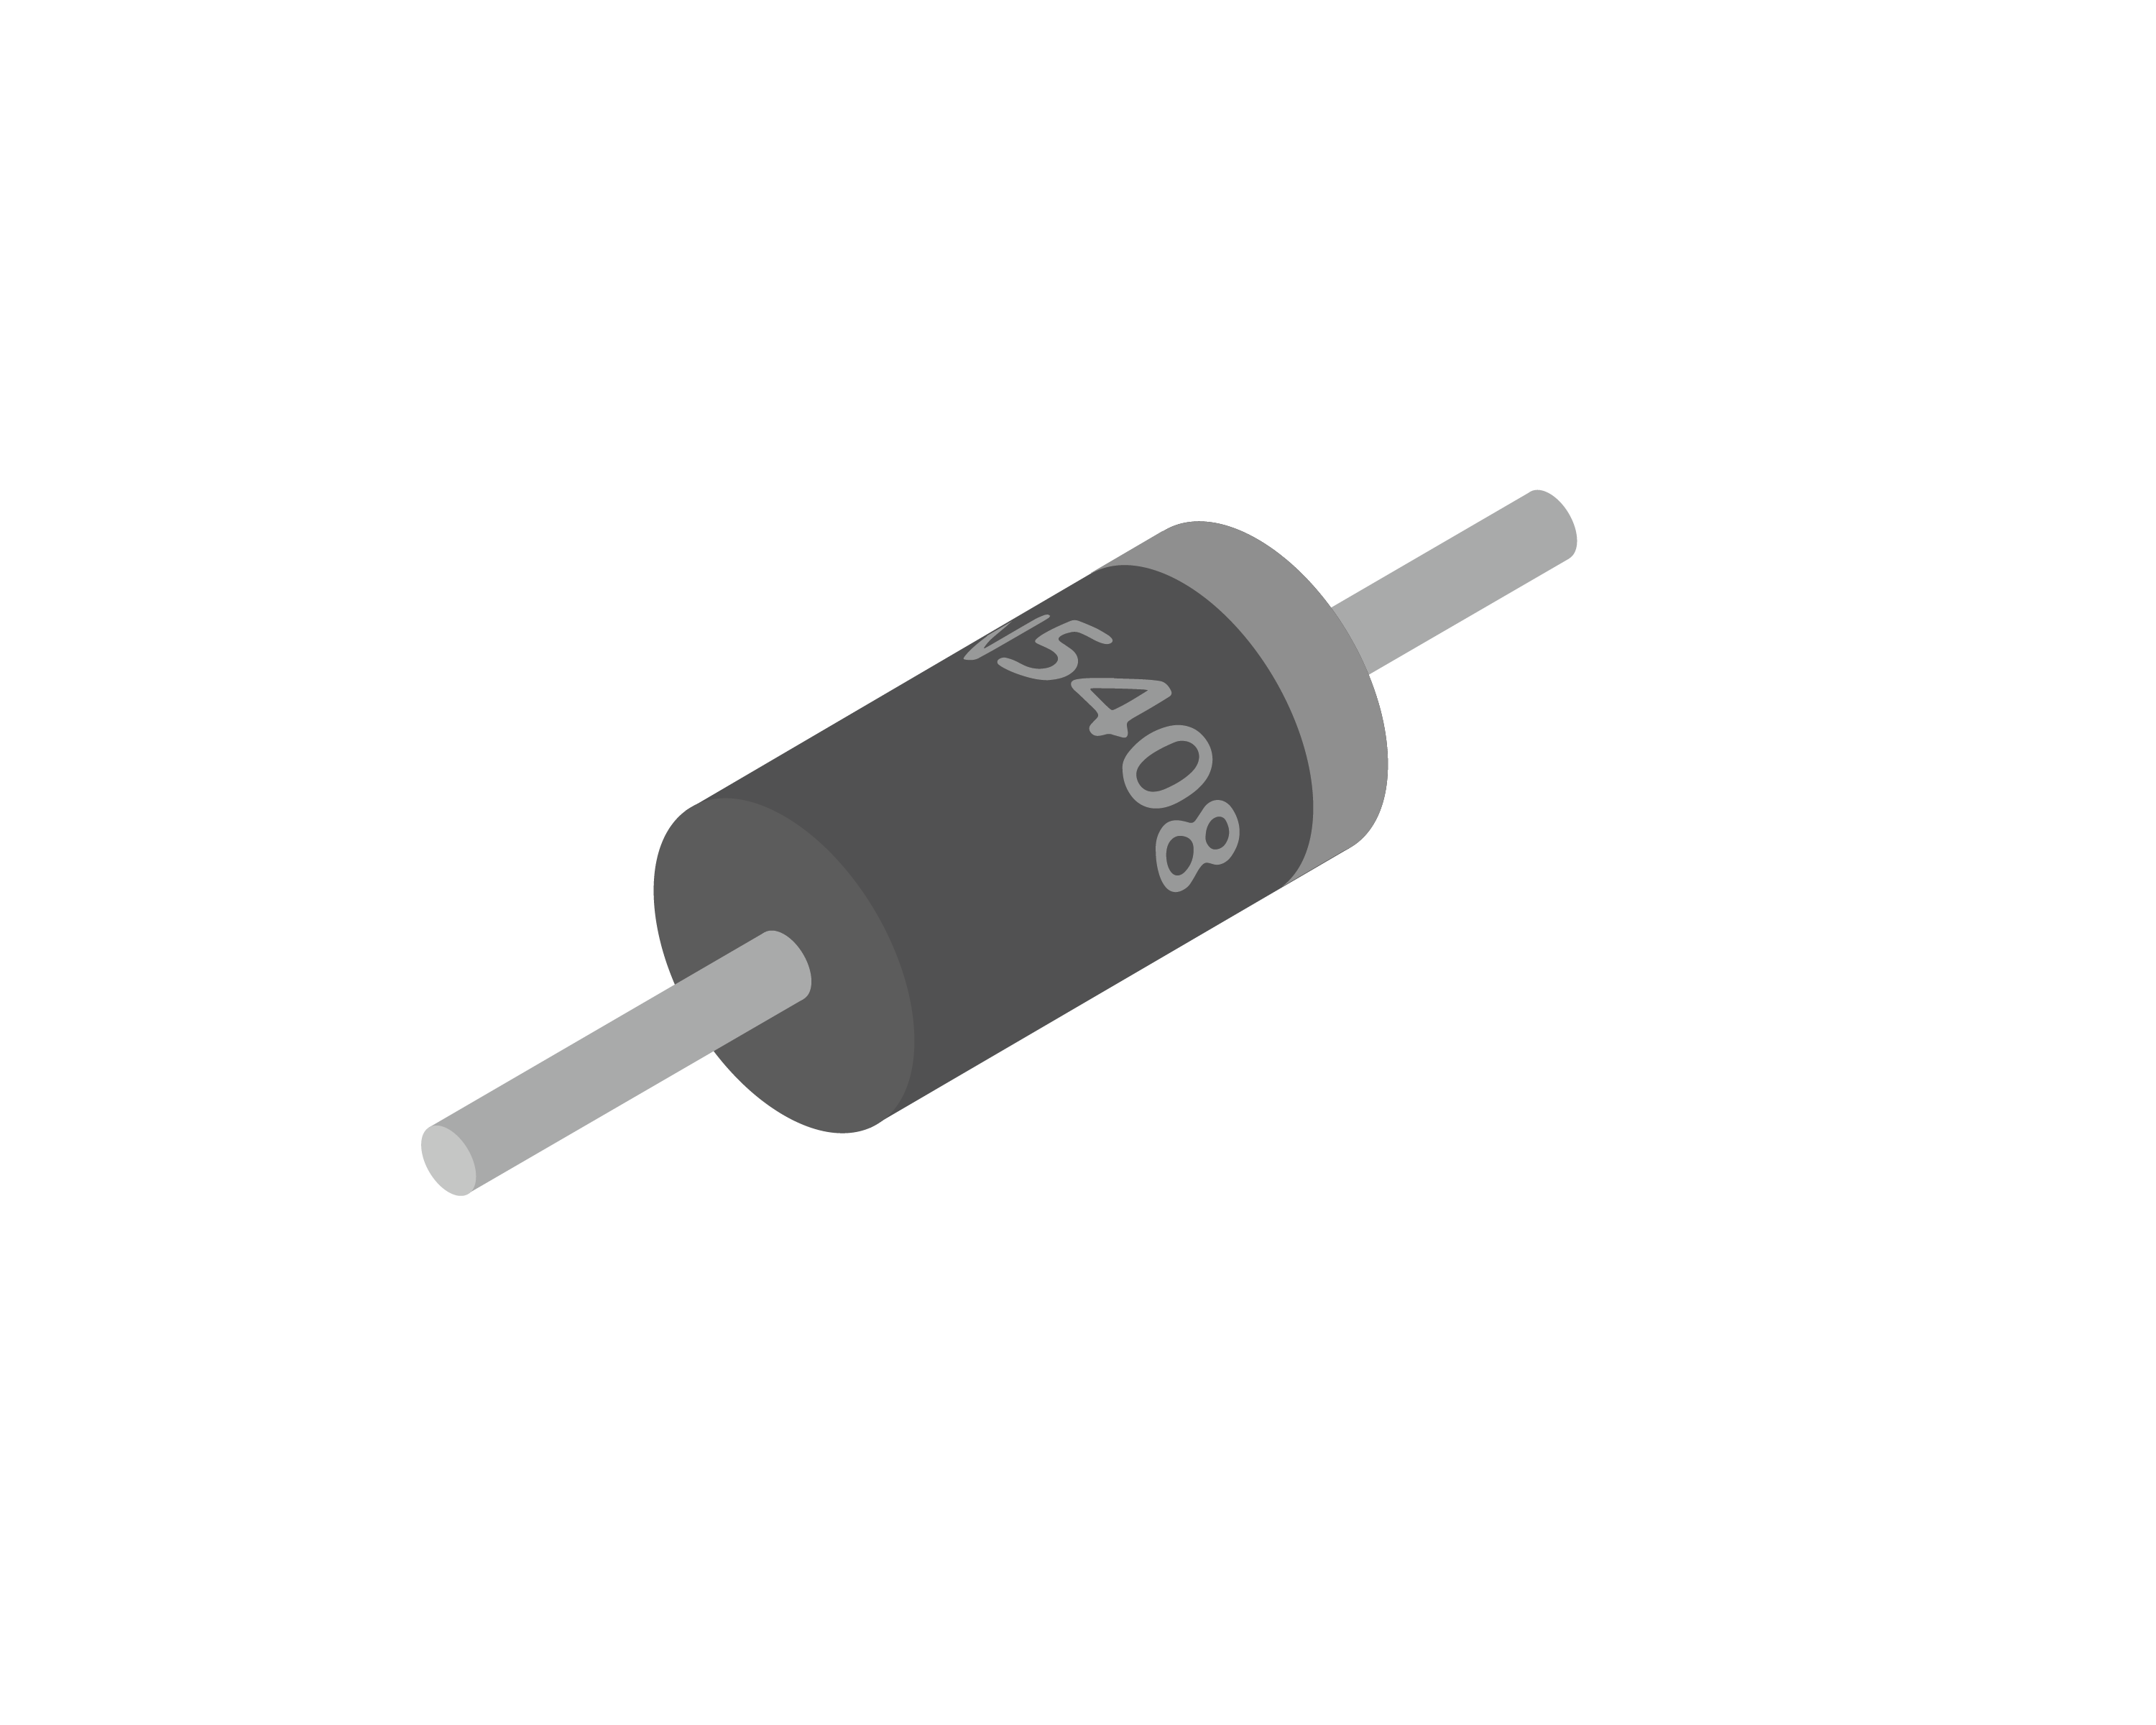
\includegraphics[width=.75\textwidth]{diodeReal.png}

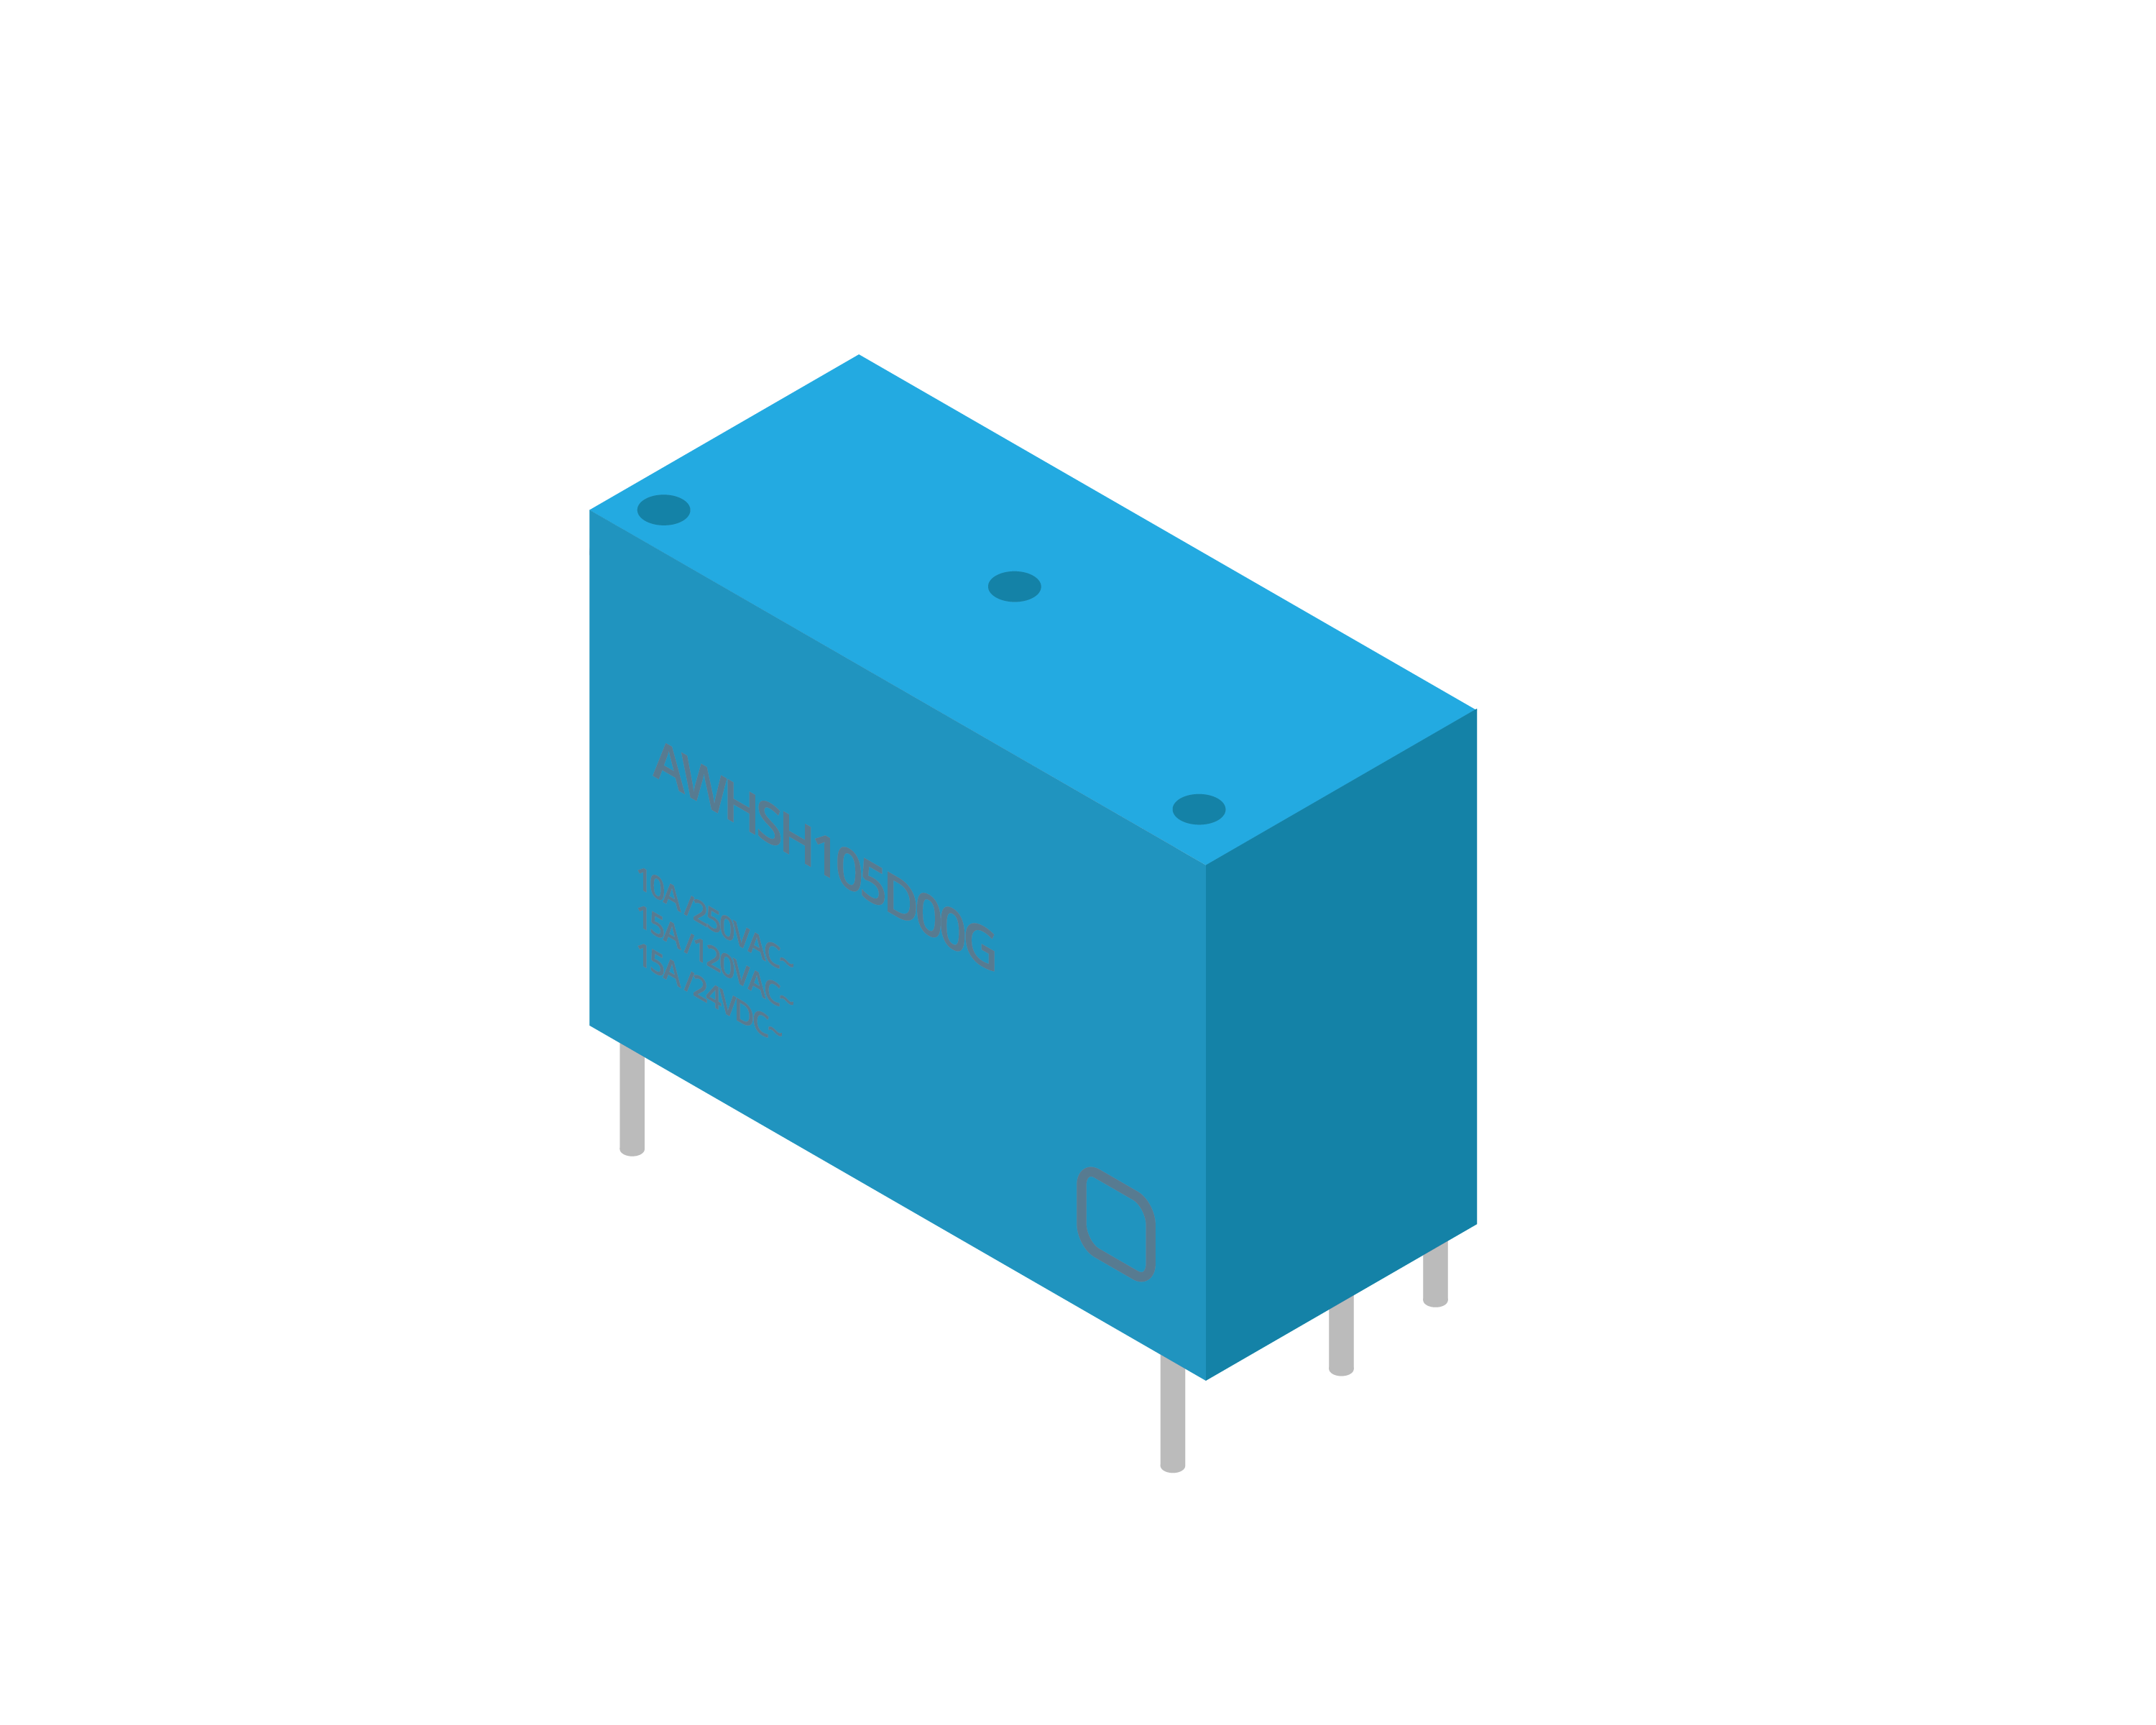
\includegraphics[width=.75\textwidth]{relayReal.png}

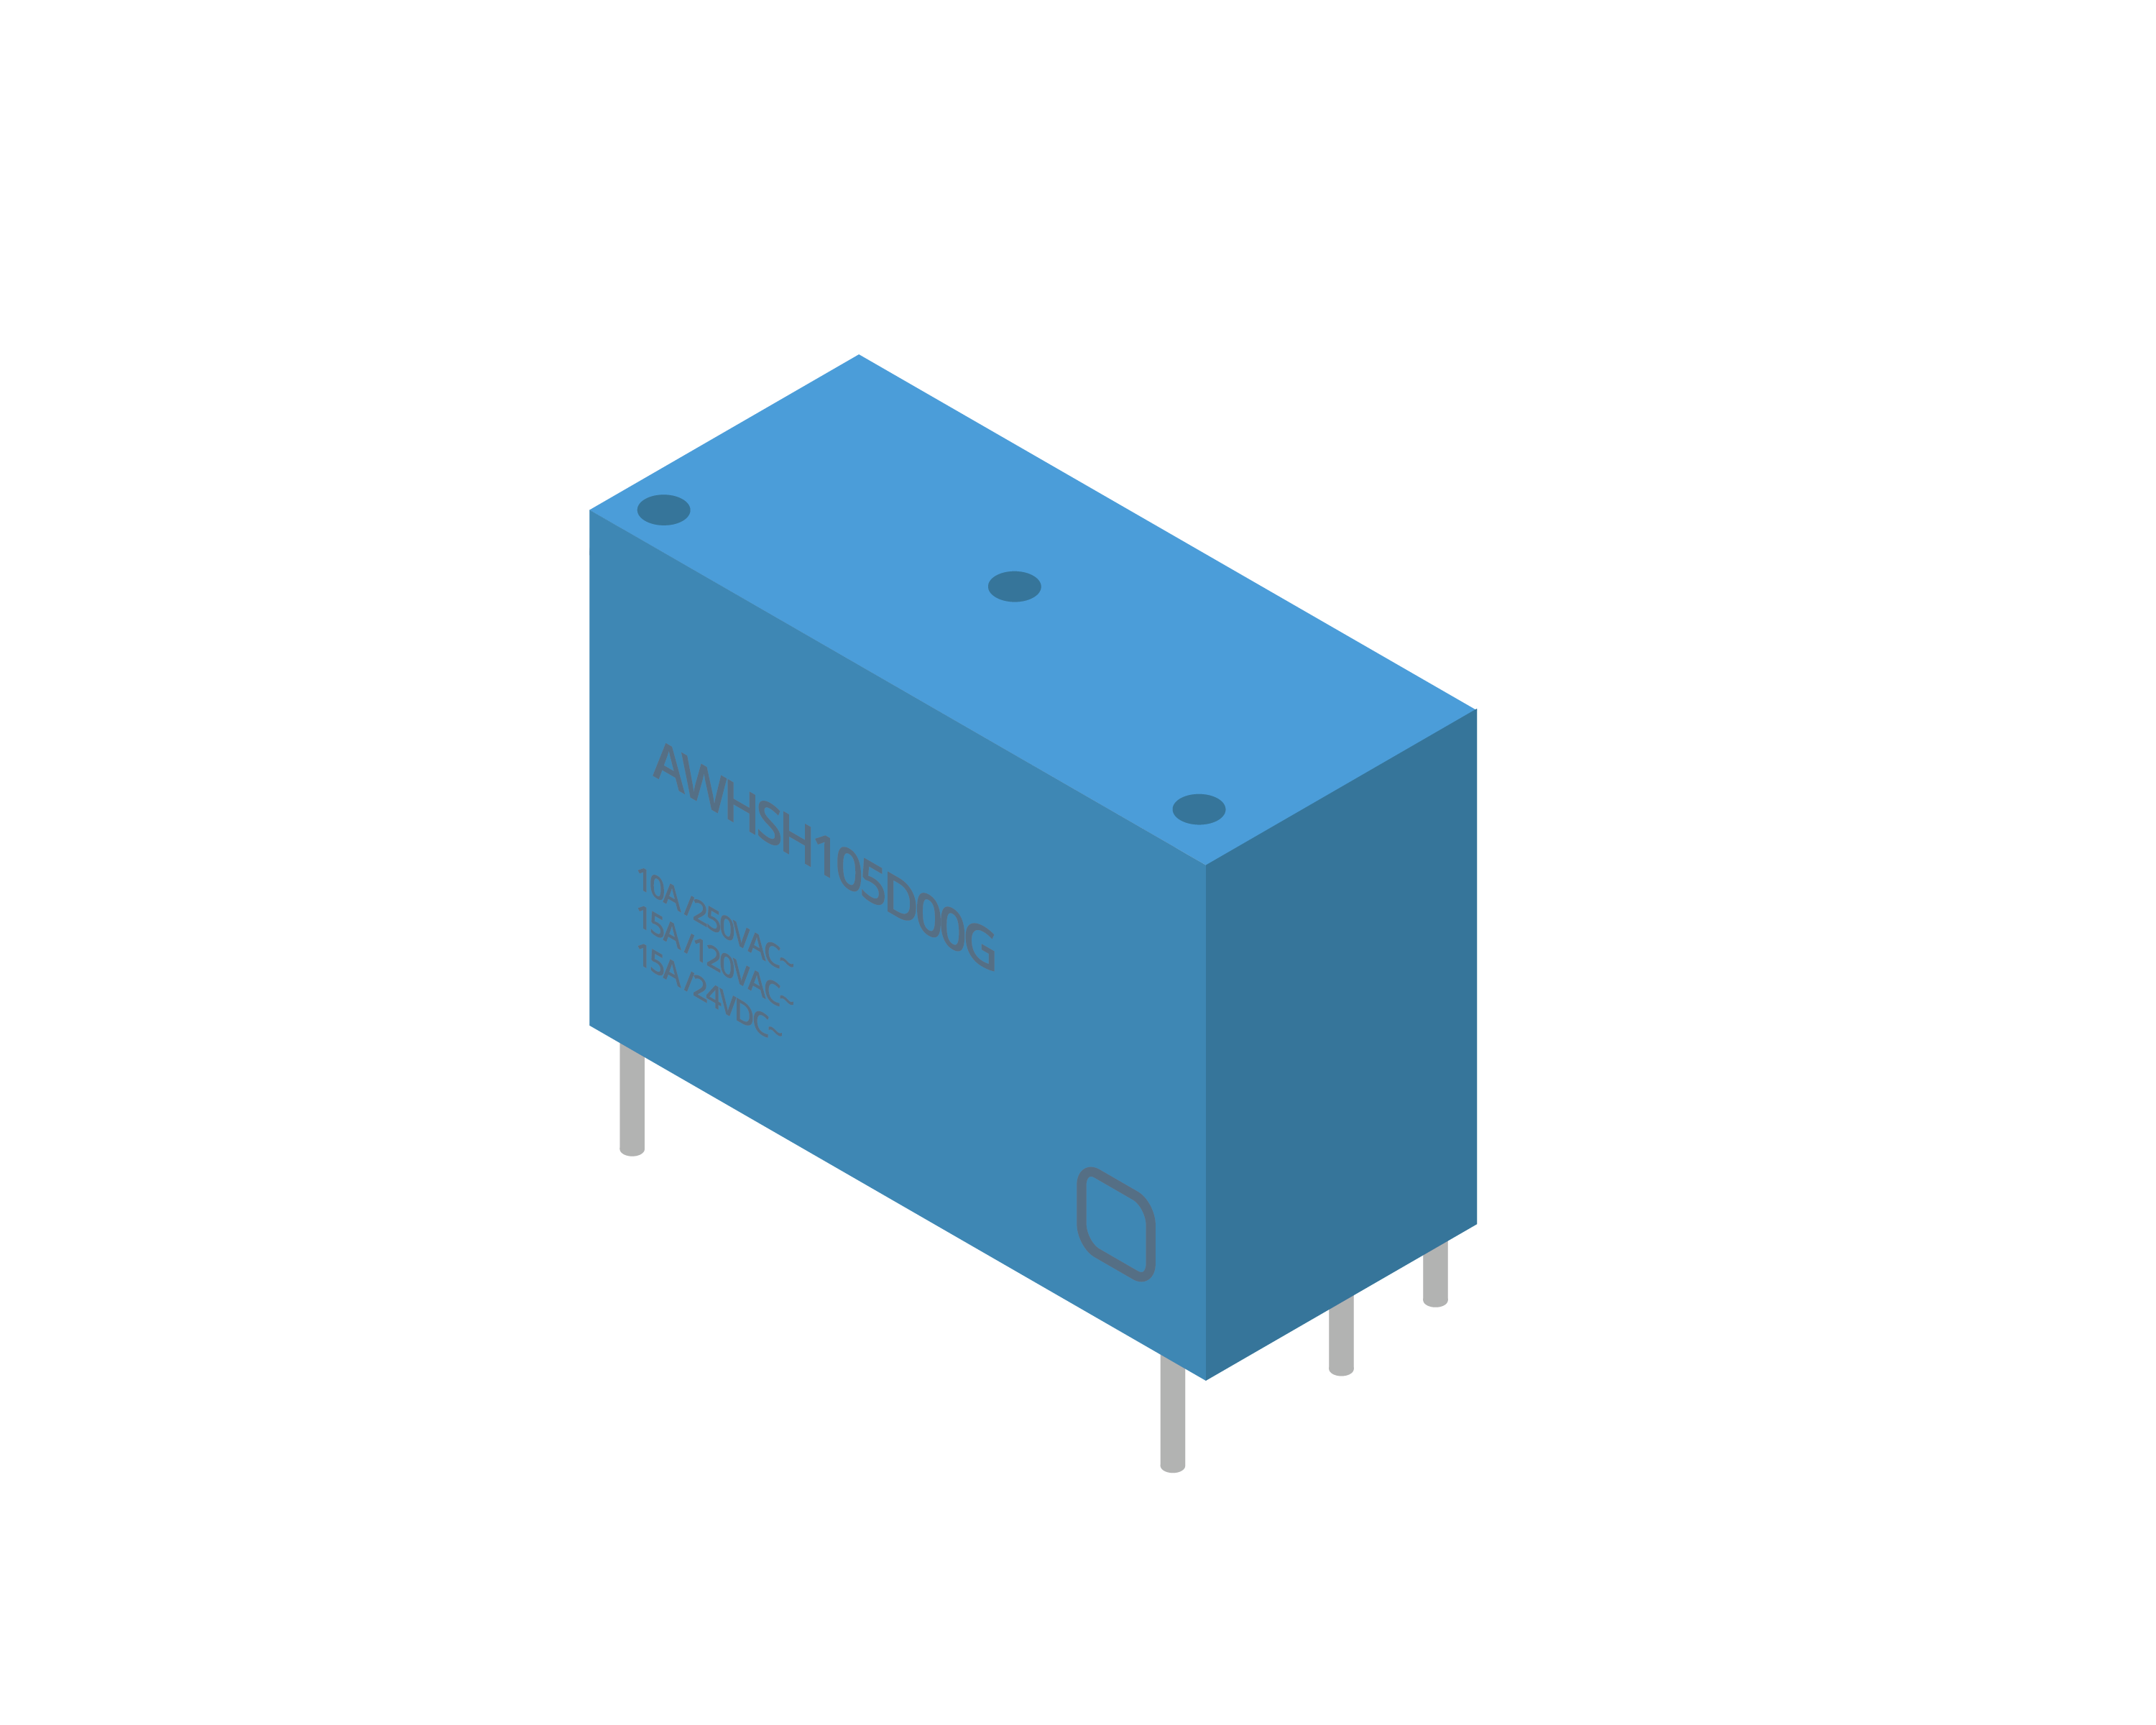
\includegraphics[width=.75\textwidth]{transistorReal.png}


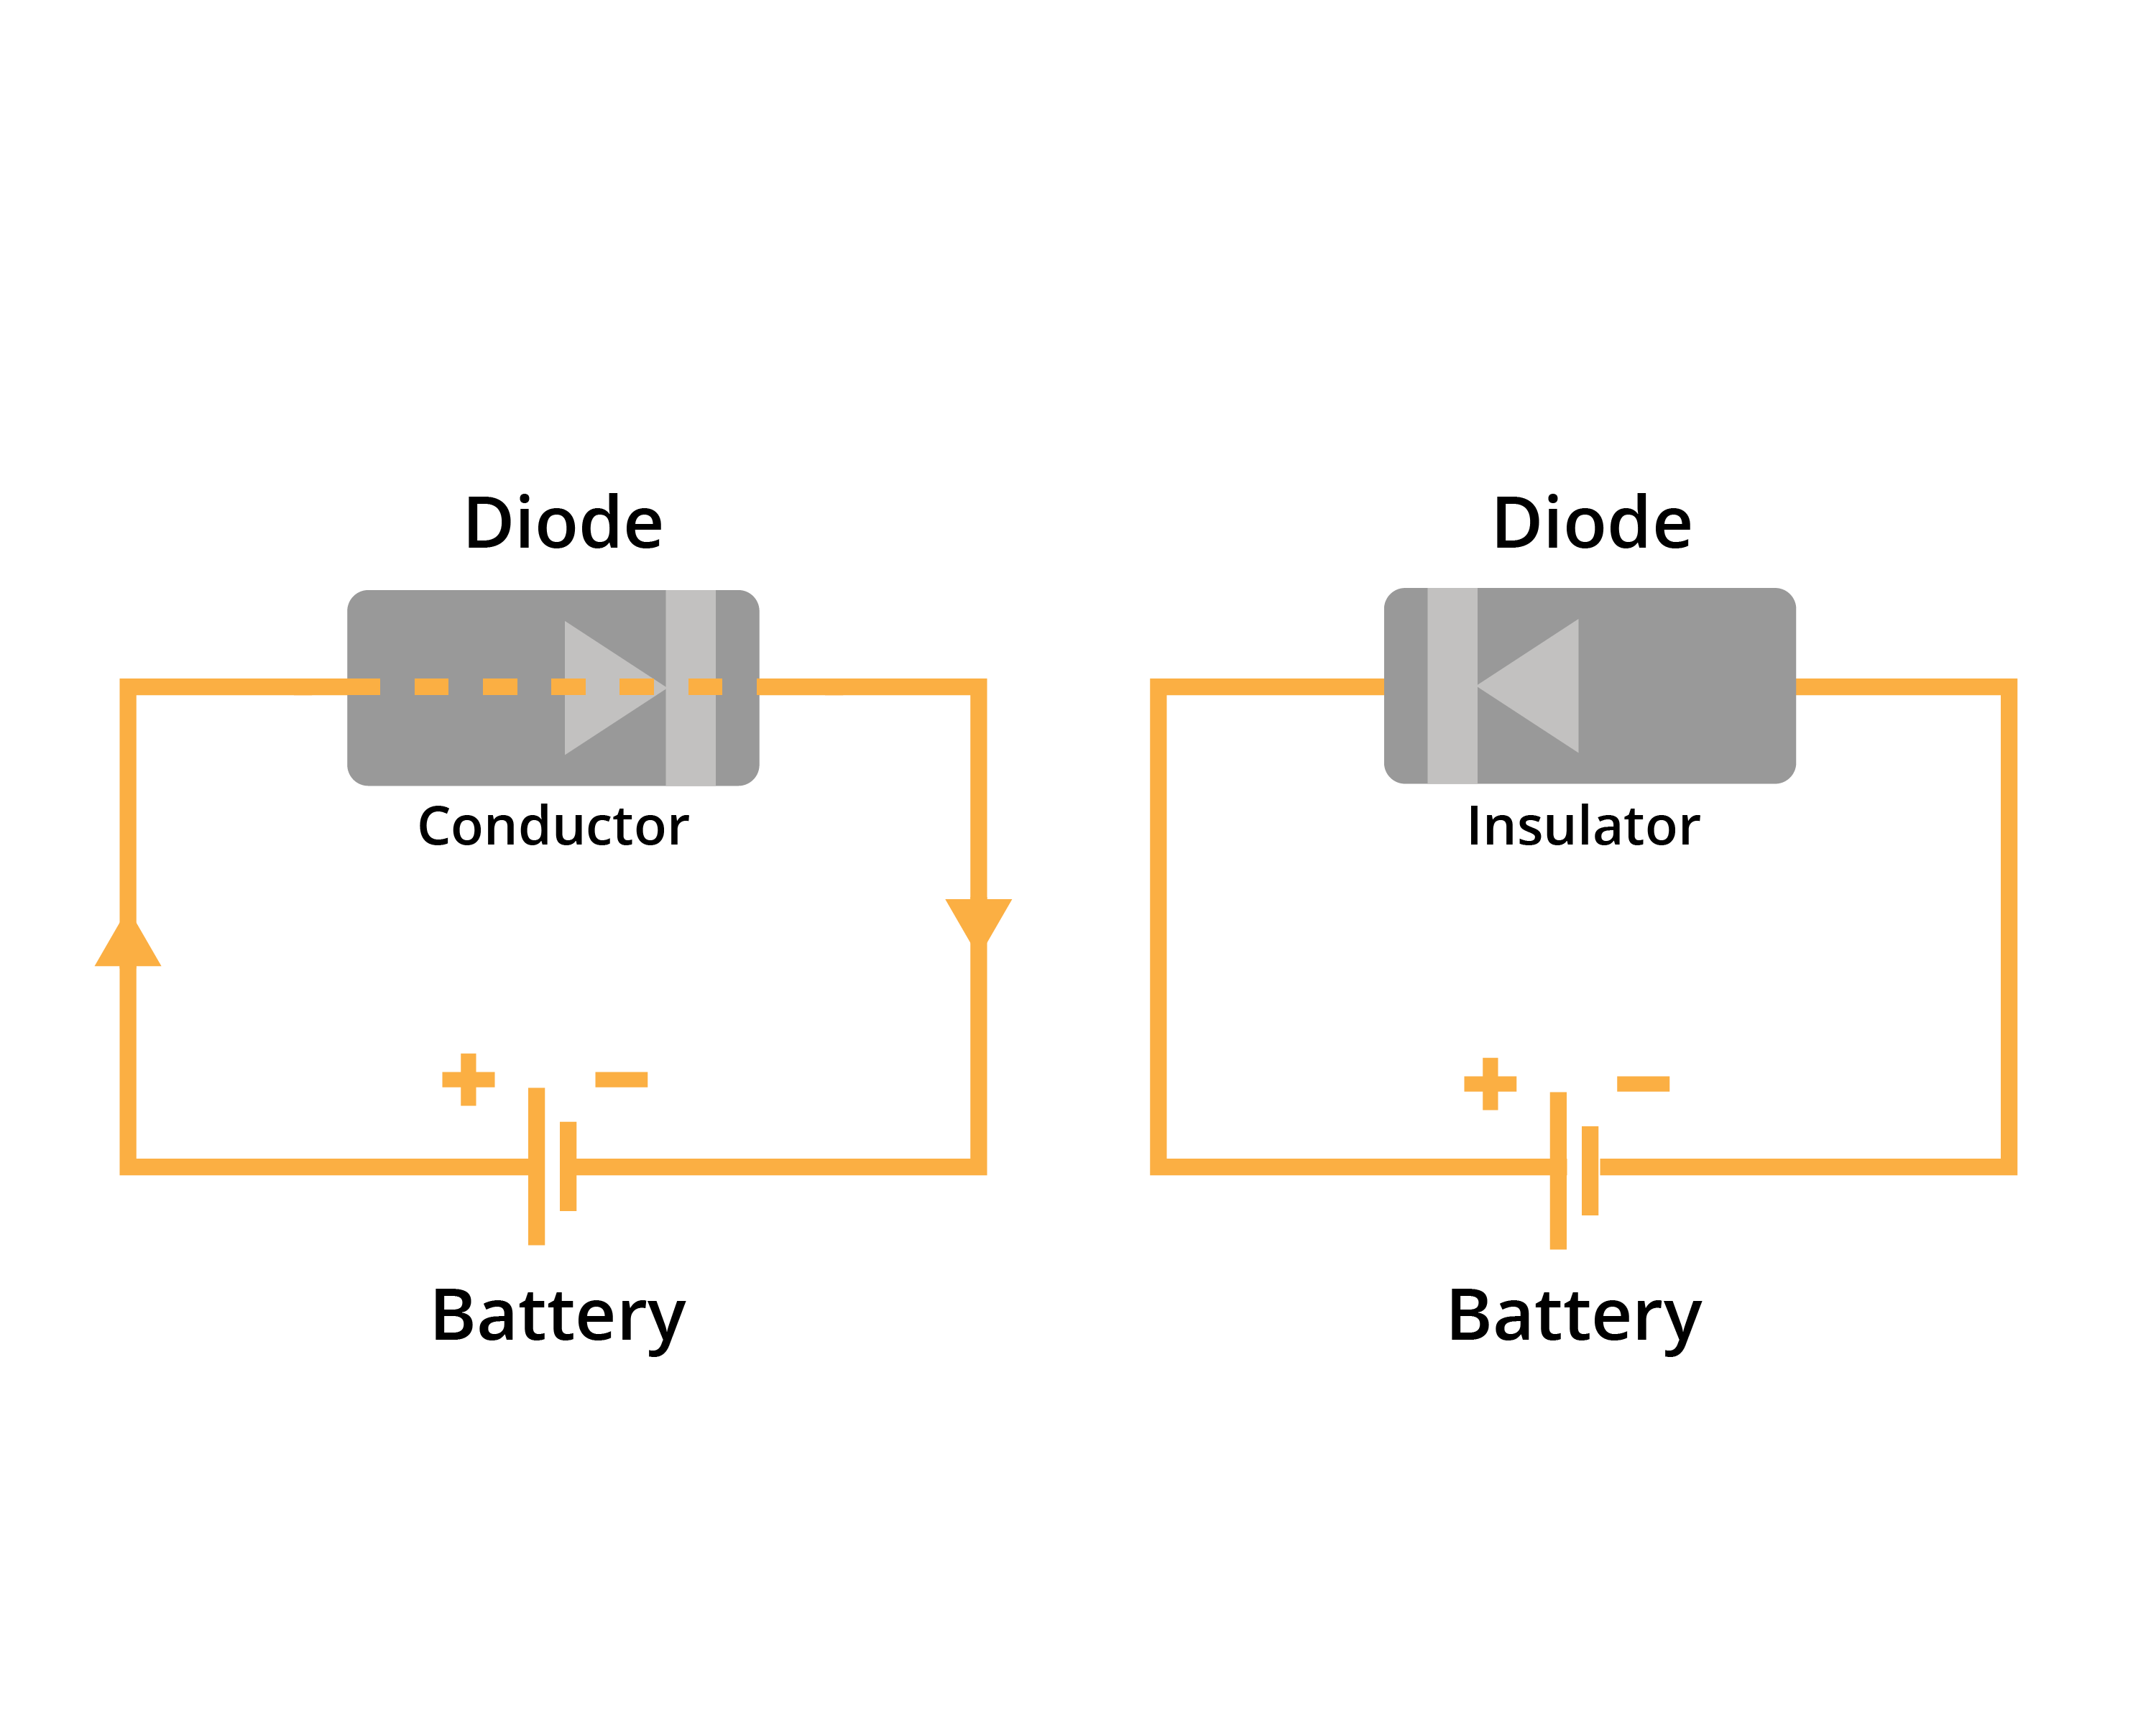
\includegraphics[width=.75\textwidth]{diodeIntroAlt.png}


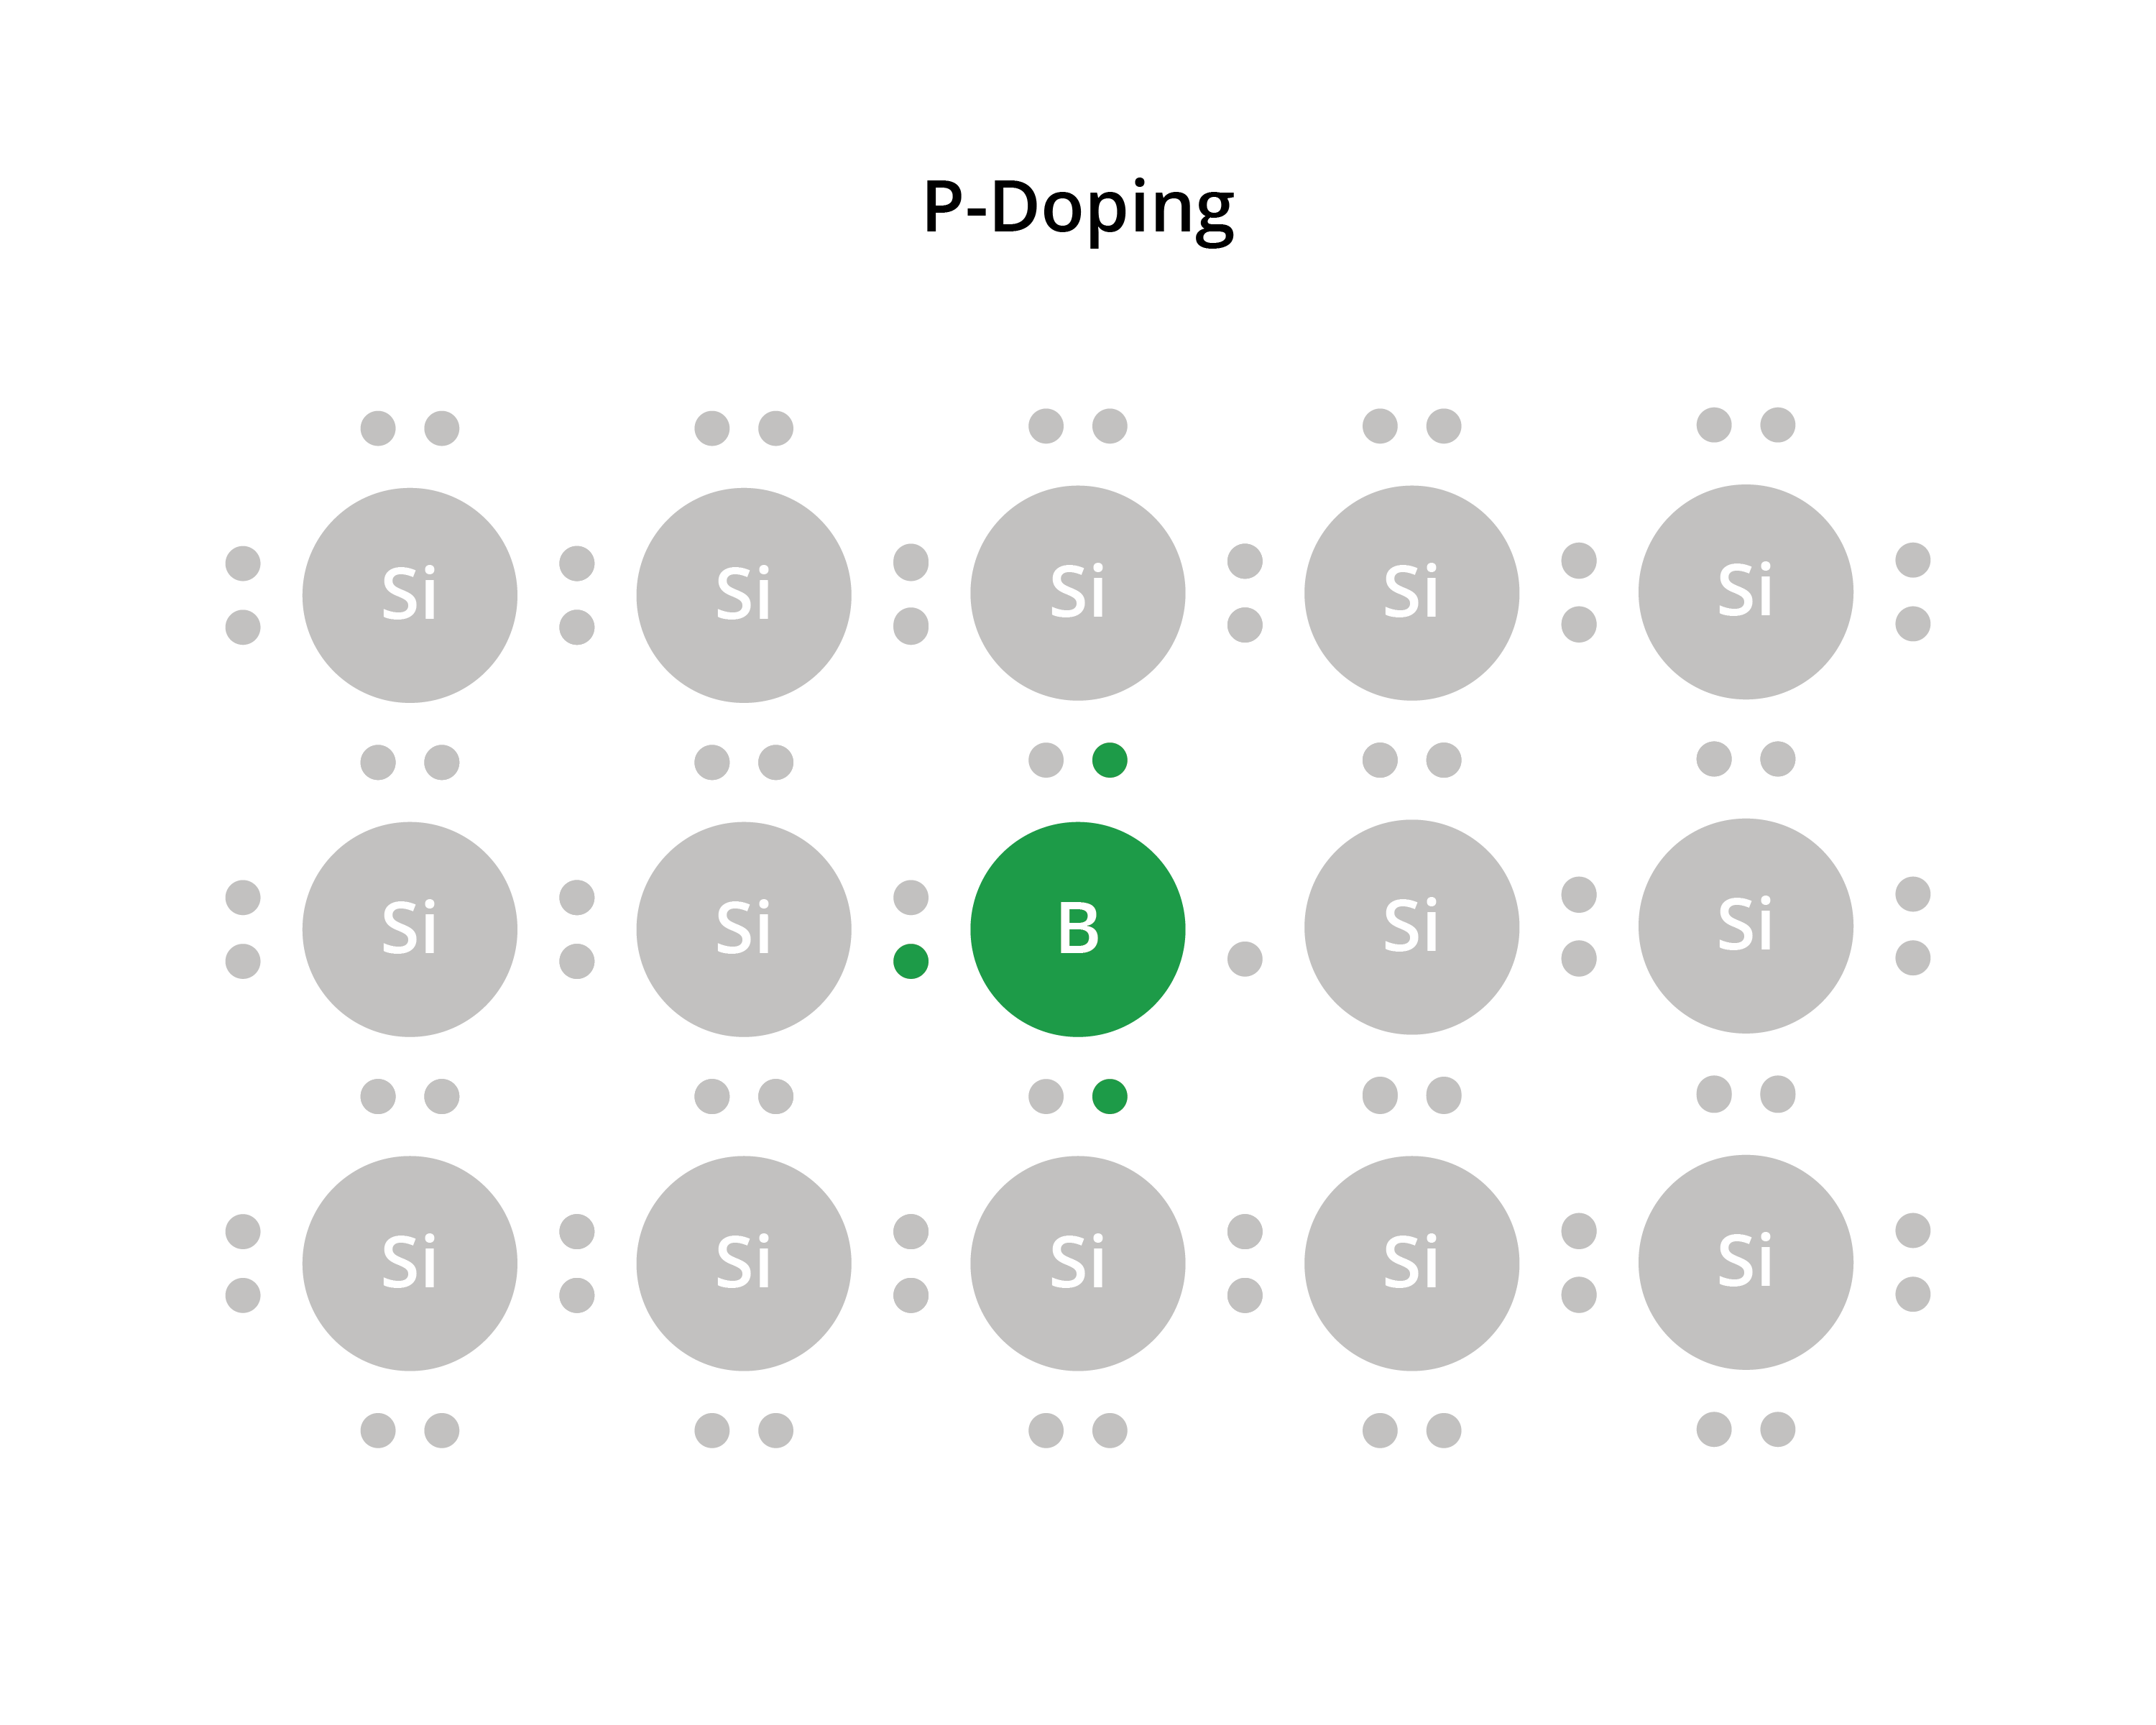
\includegraphics[width=.75\textwidth]{doping-26.png}

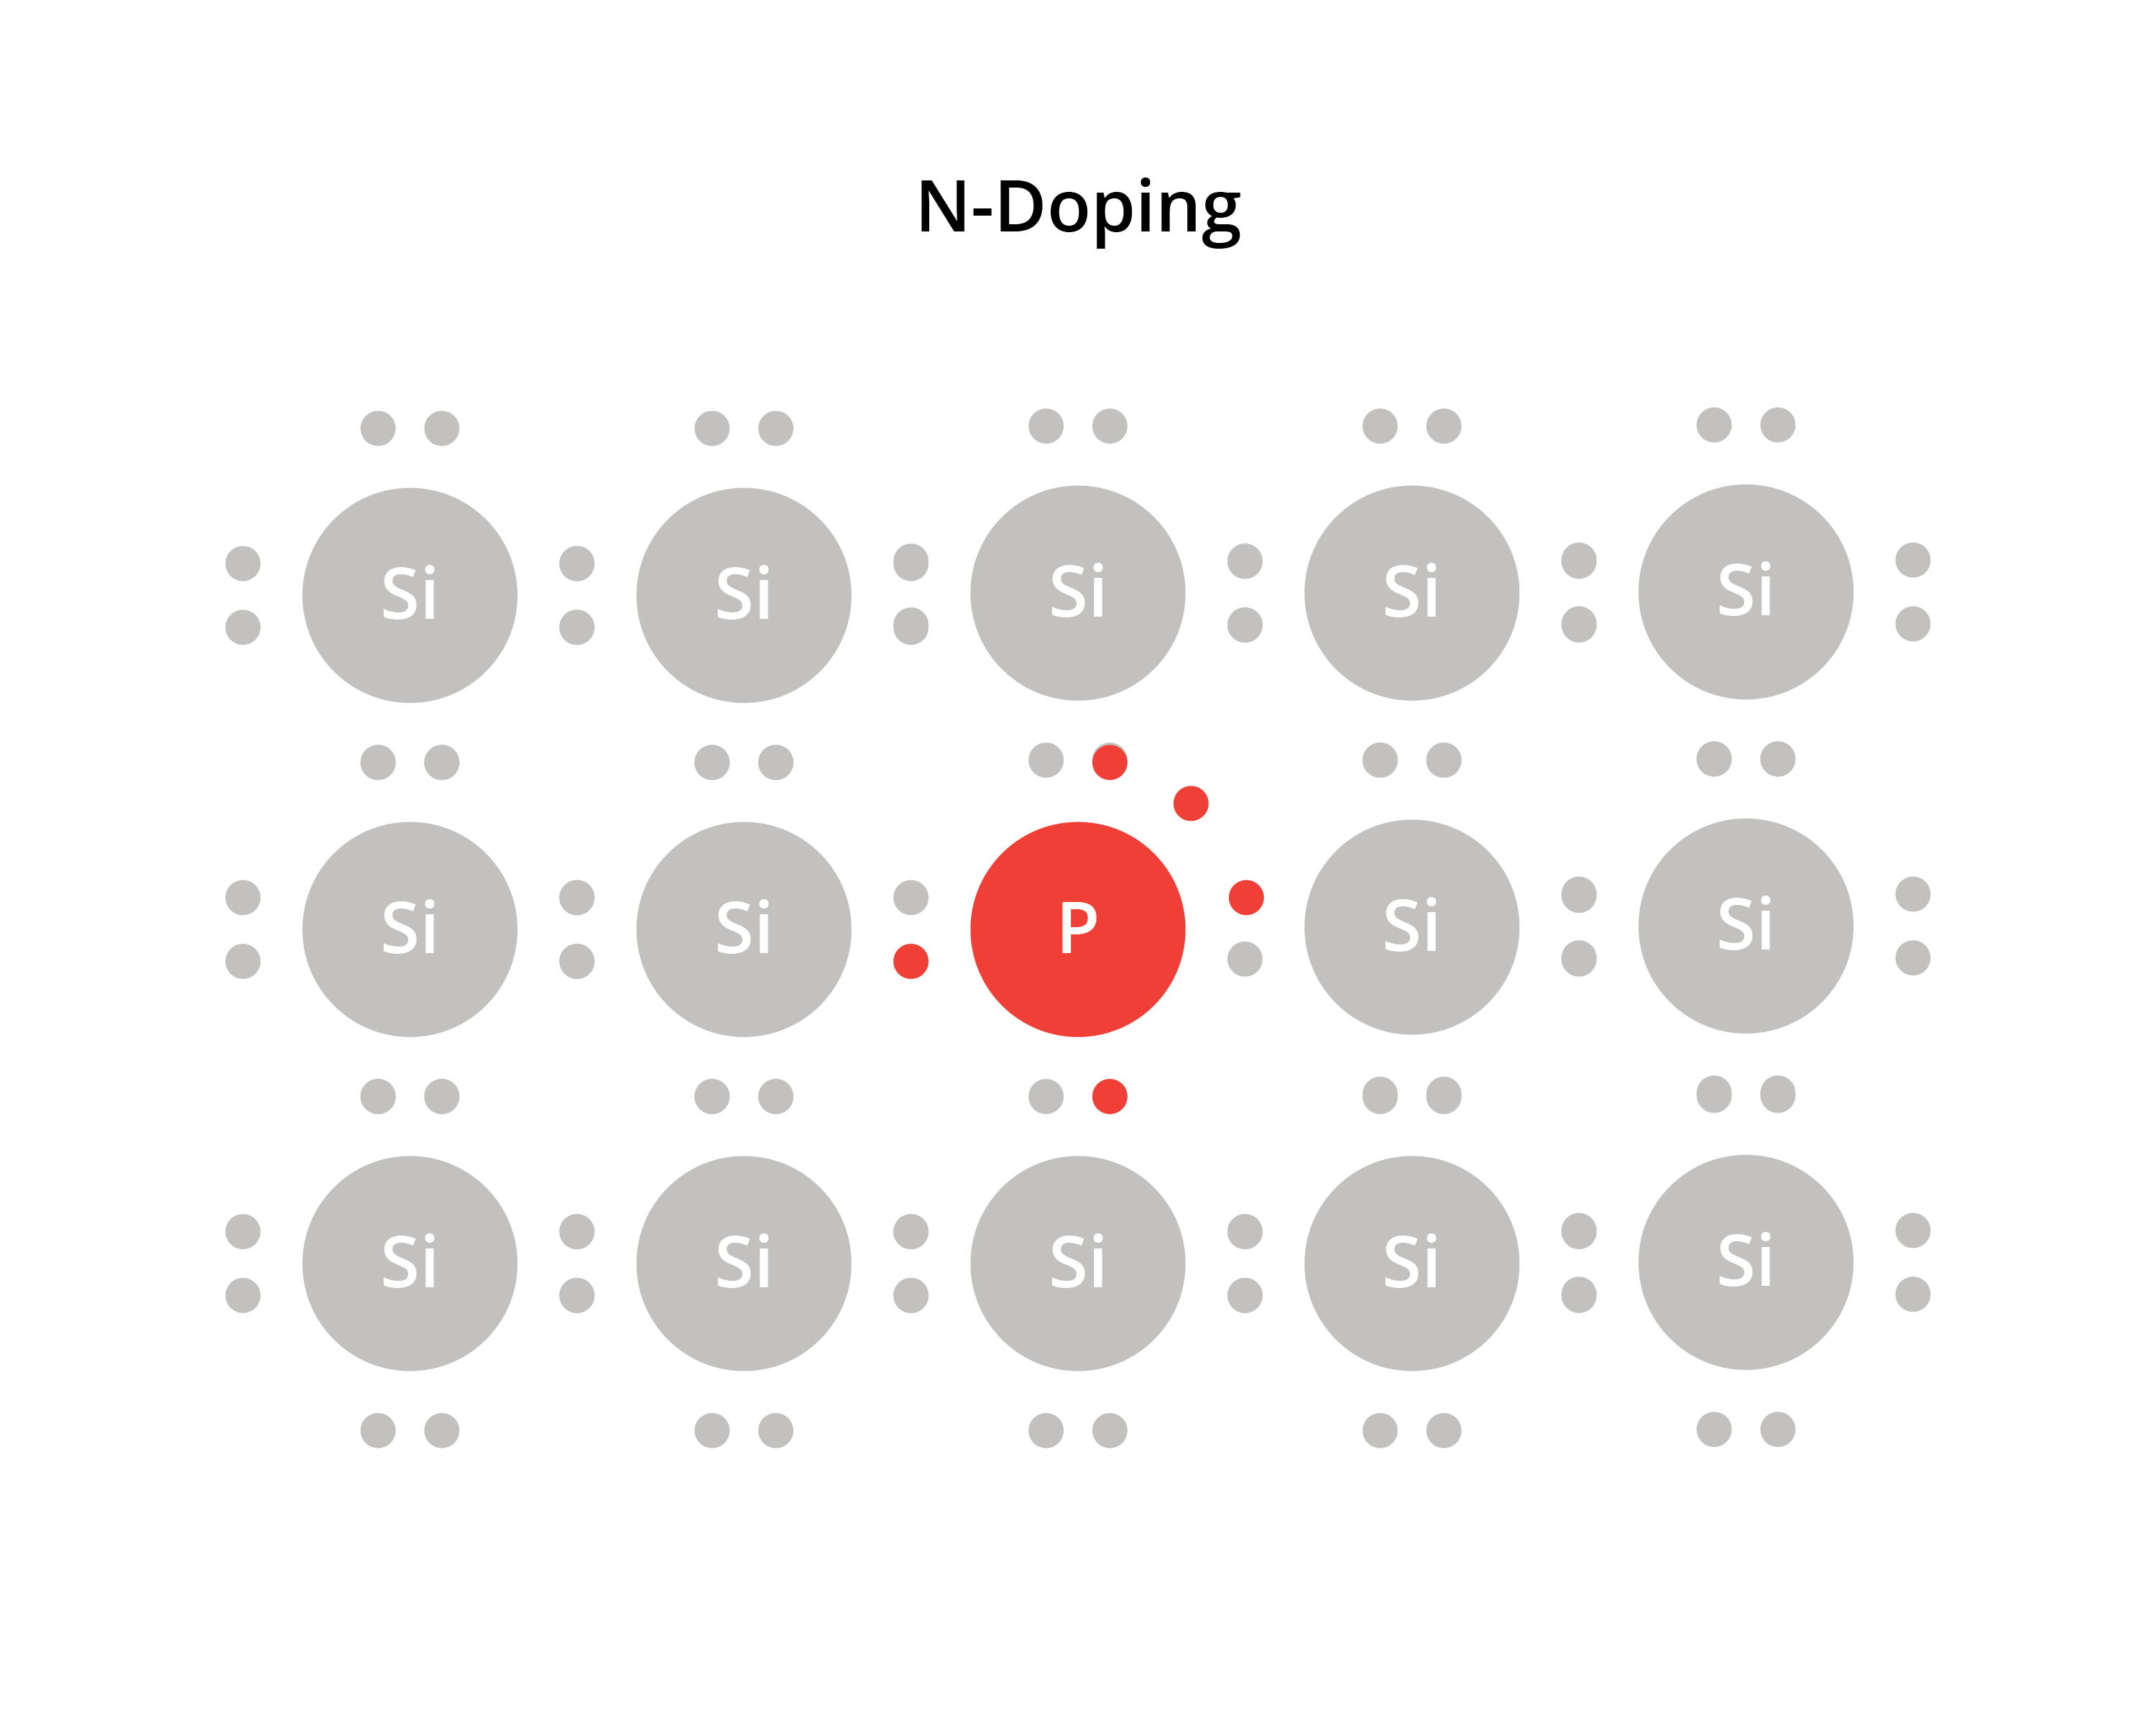
\includegraphics[width=.75\textwidth]{doping-27.png}

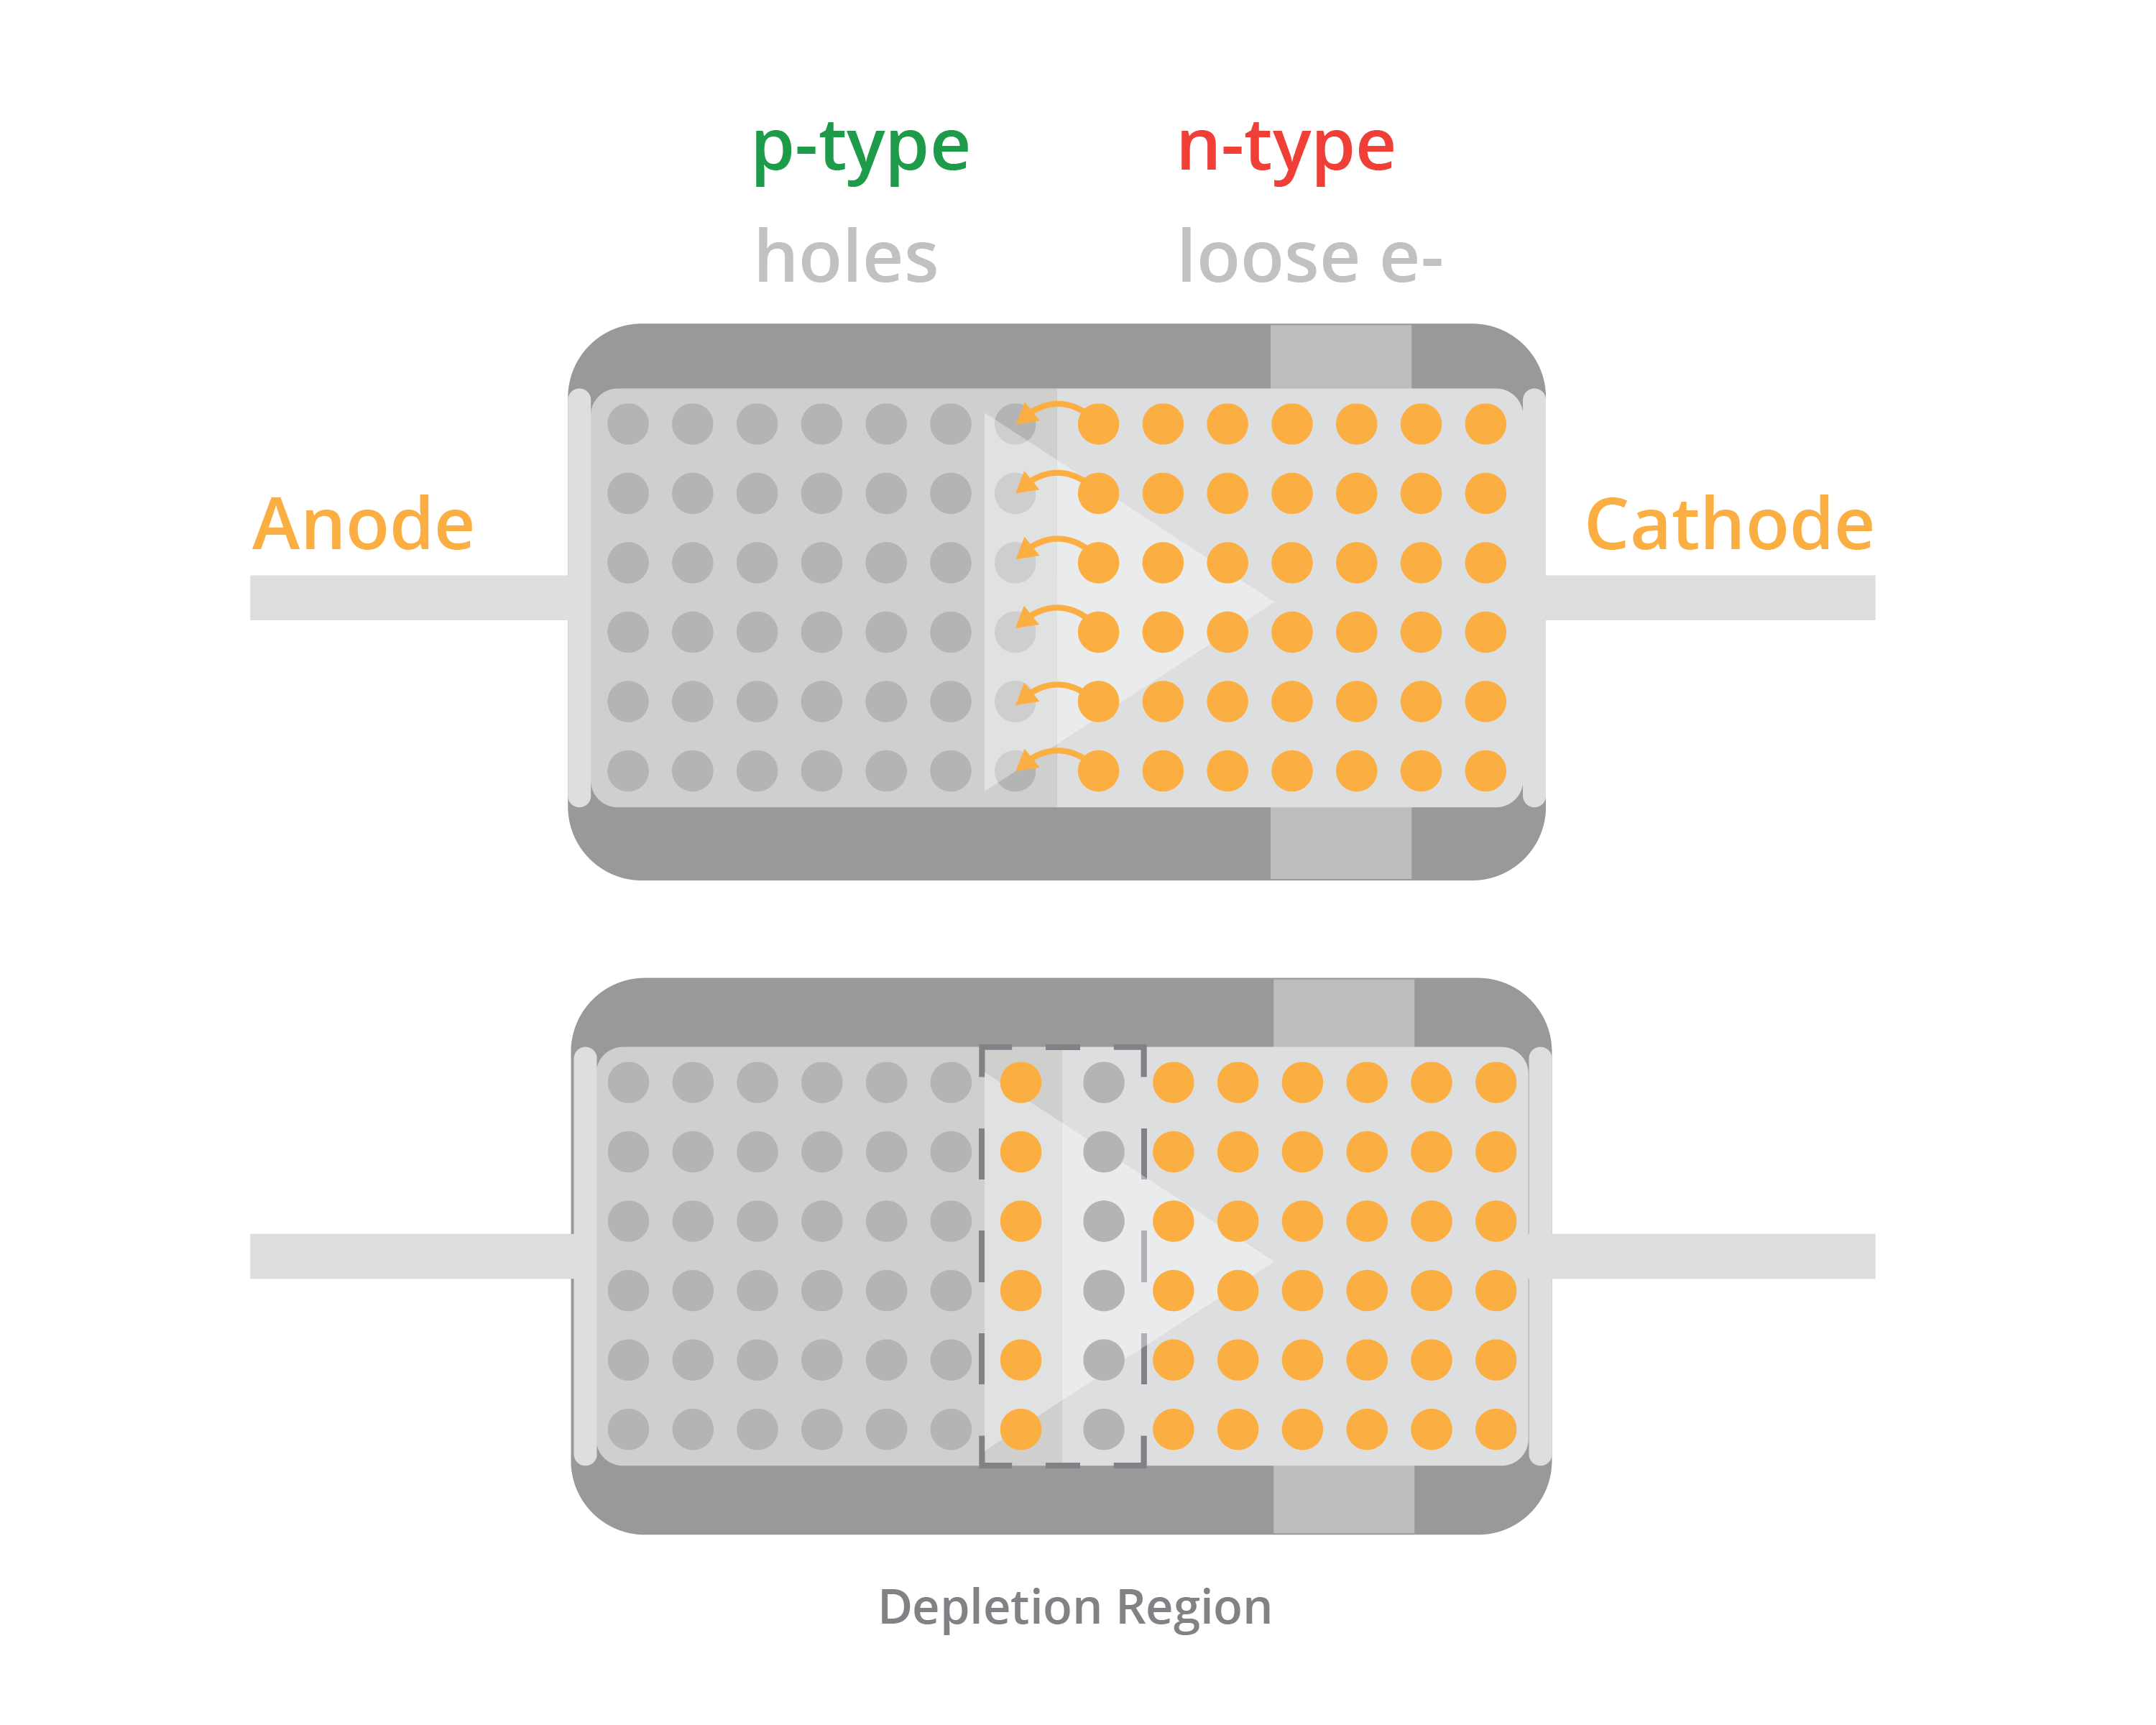
\includegraphics[width=.75\textwidth]{diodeProcess-31.png}

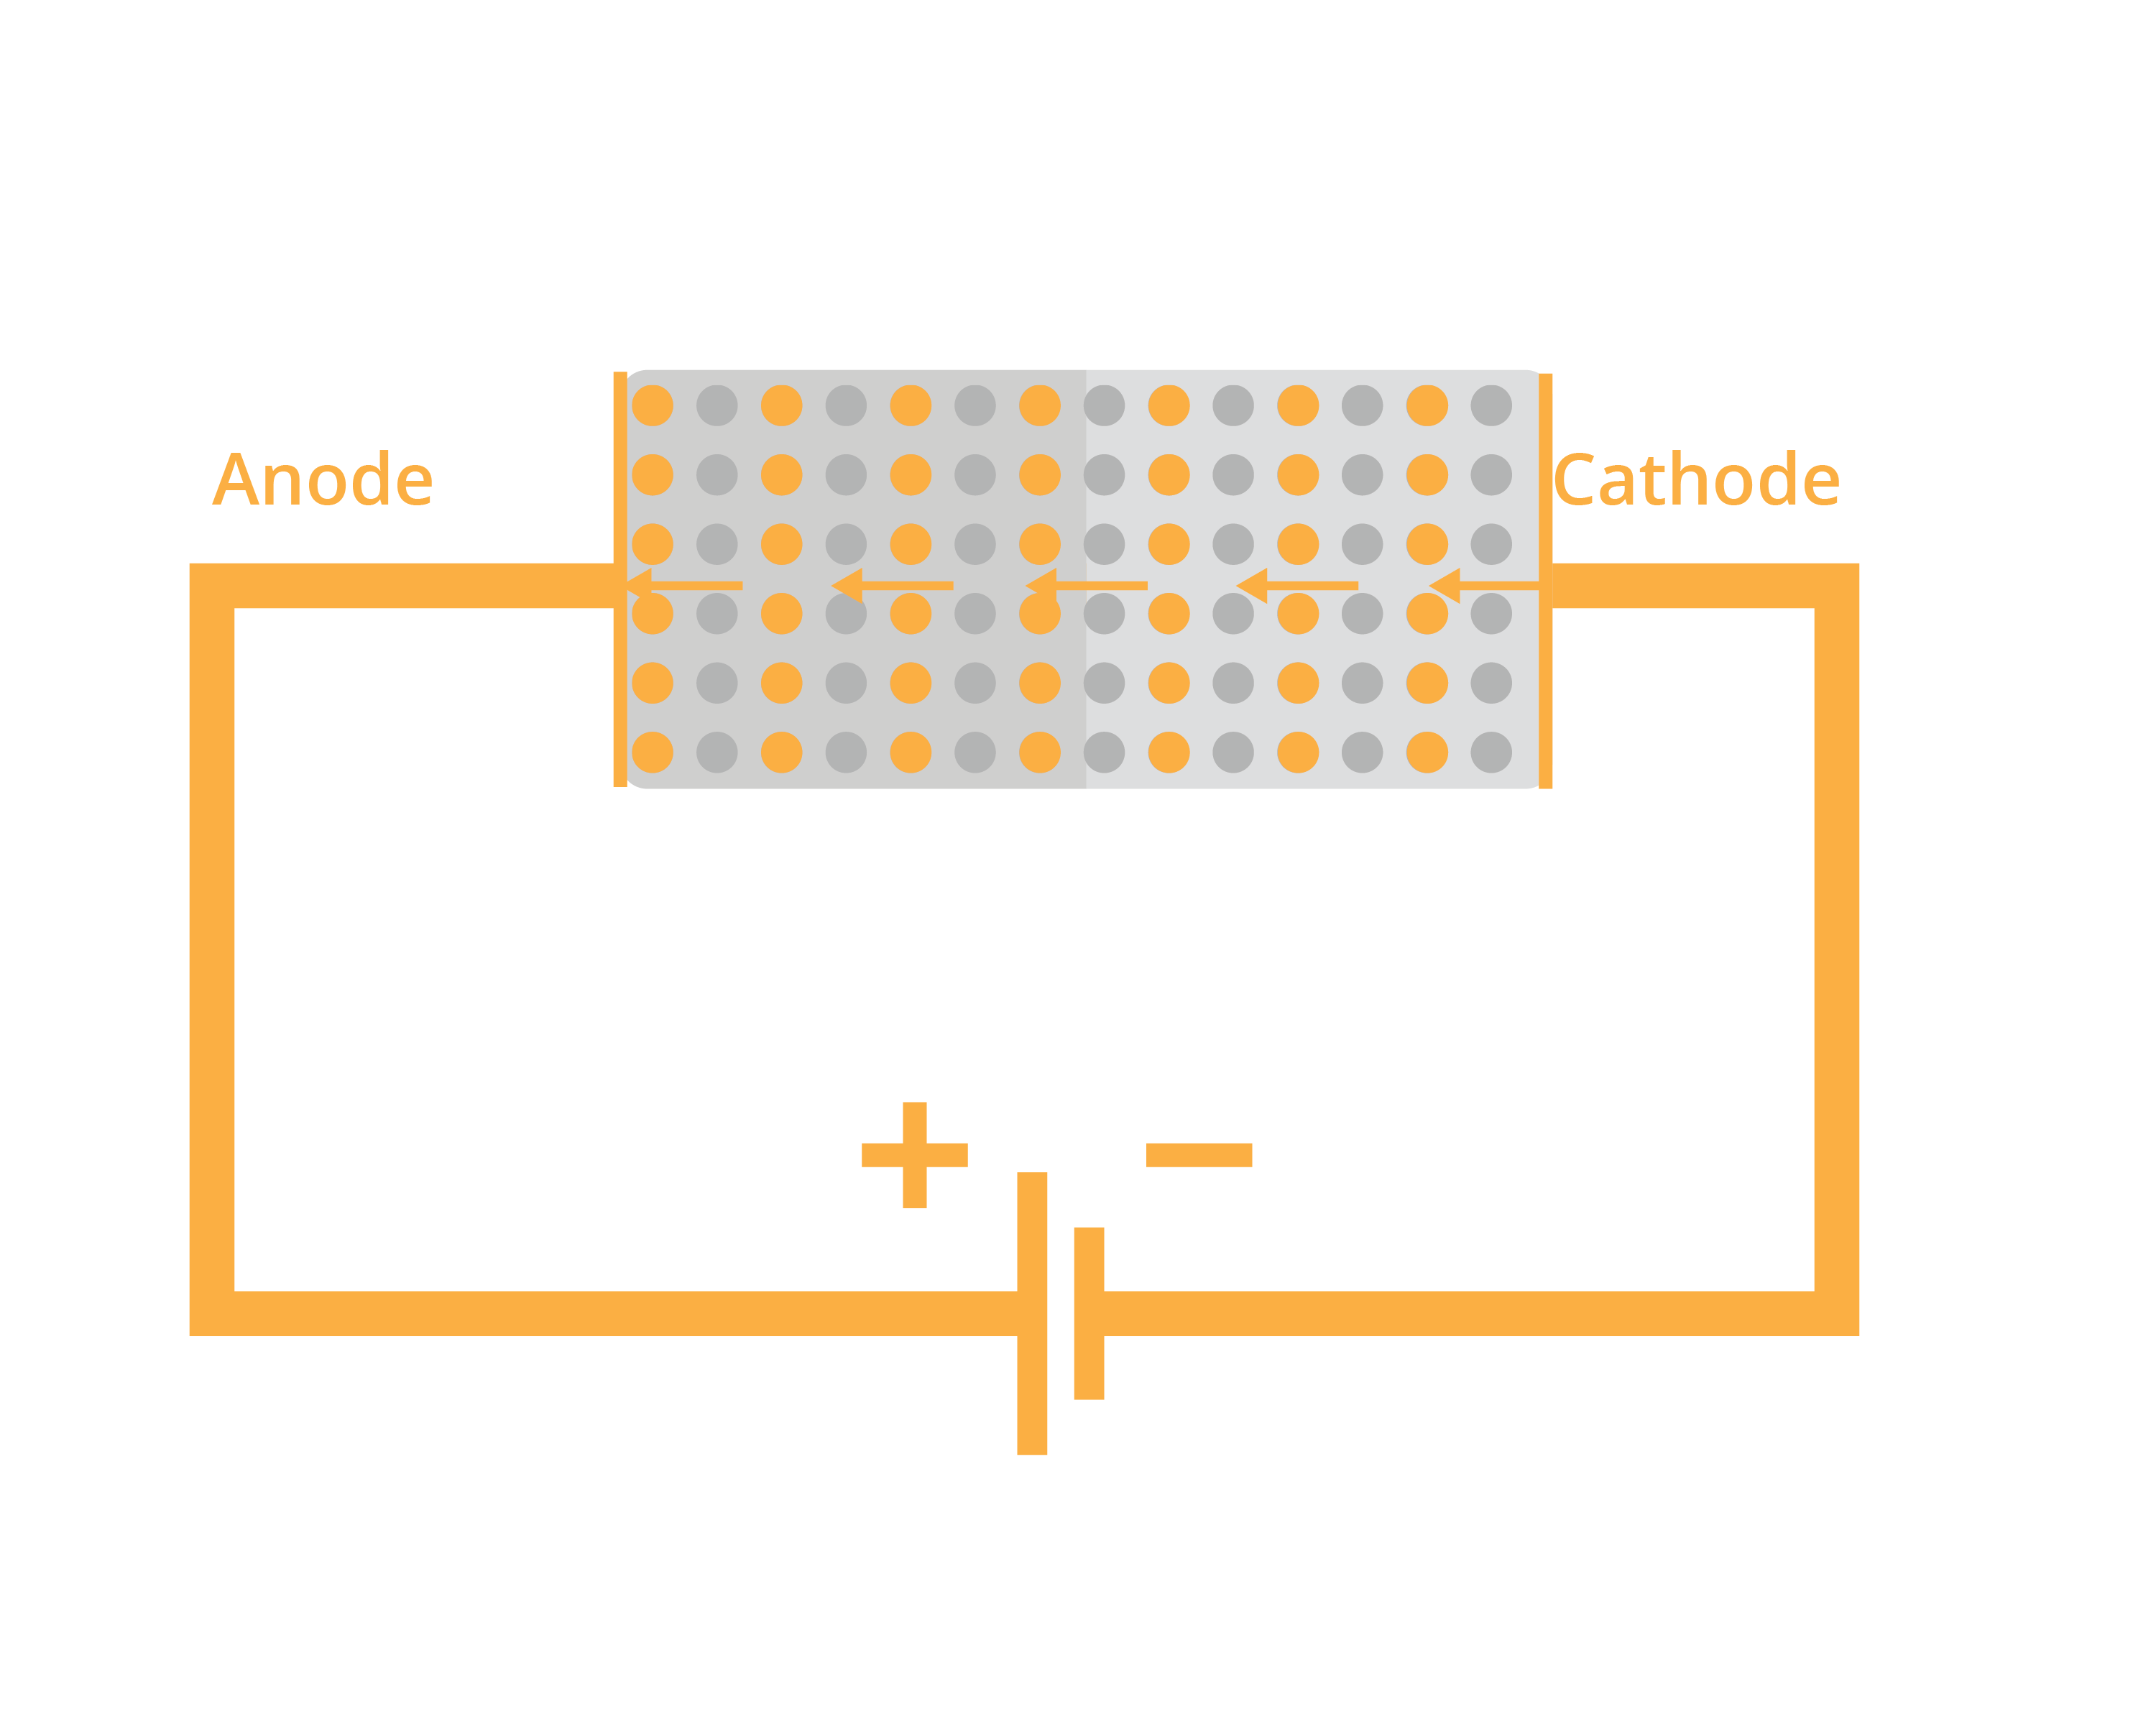
\includegraphics[width=.75\textwidth]{diodeProcess-32.png}


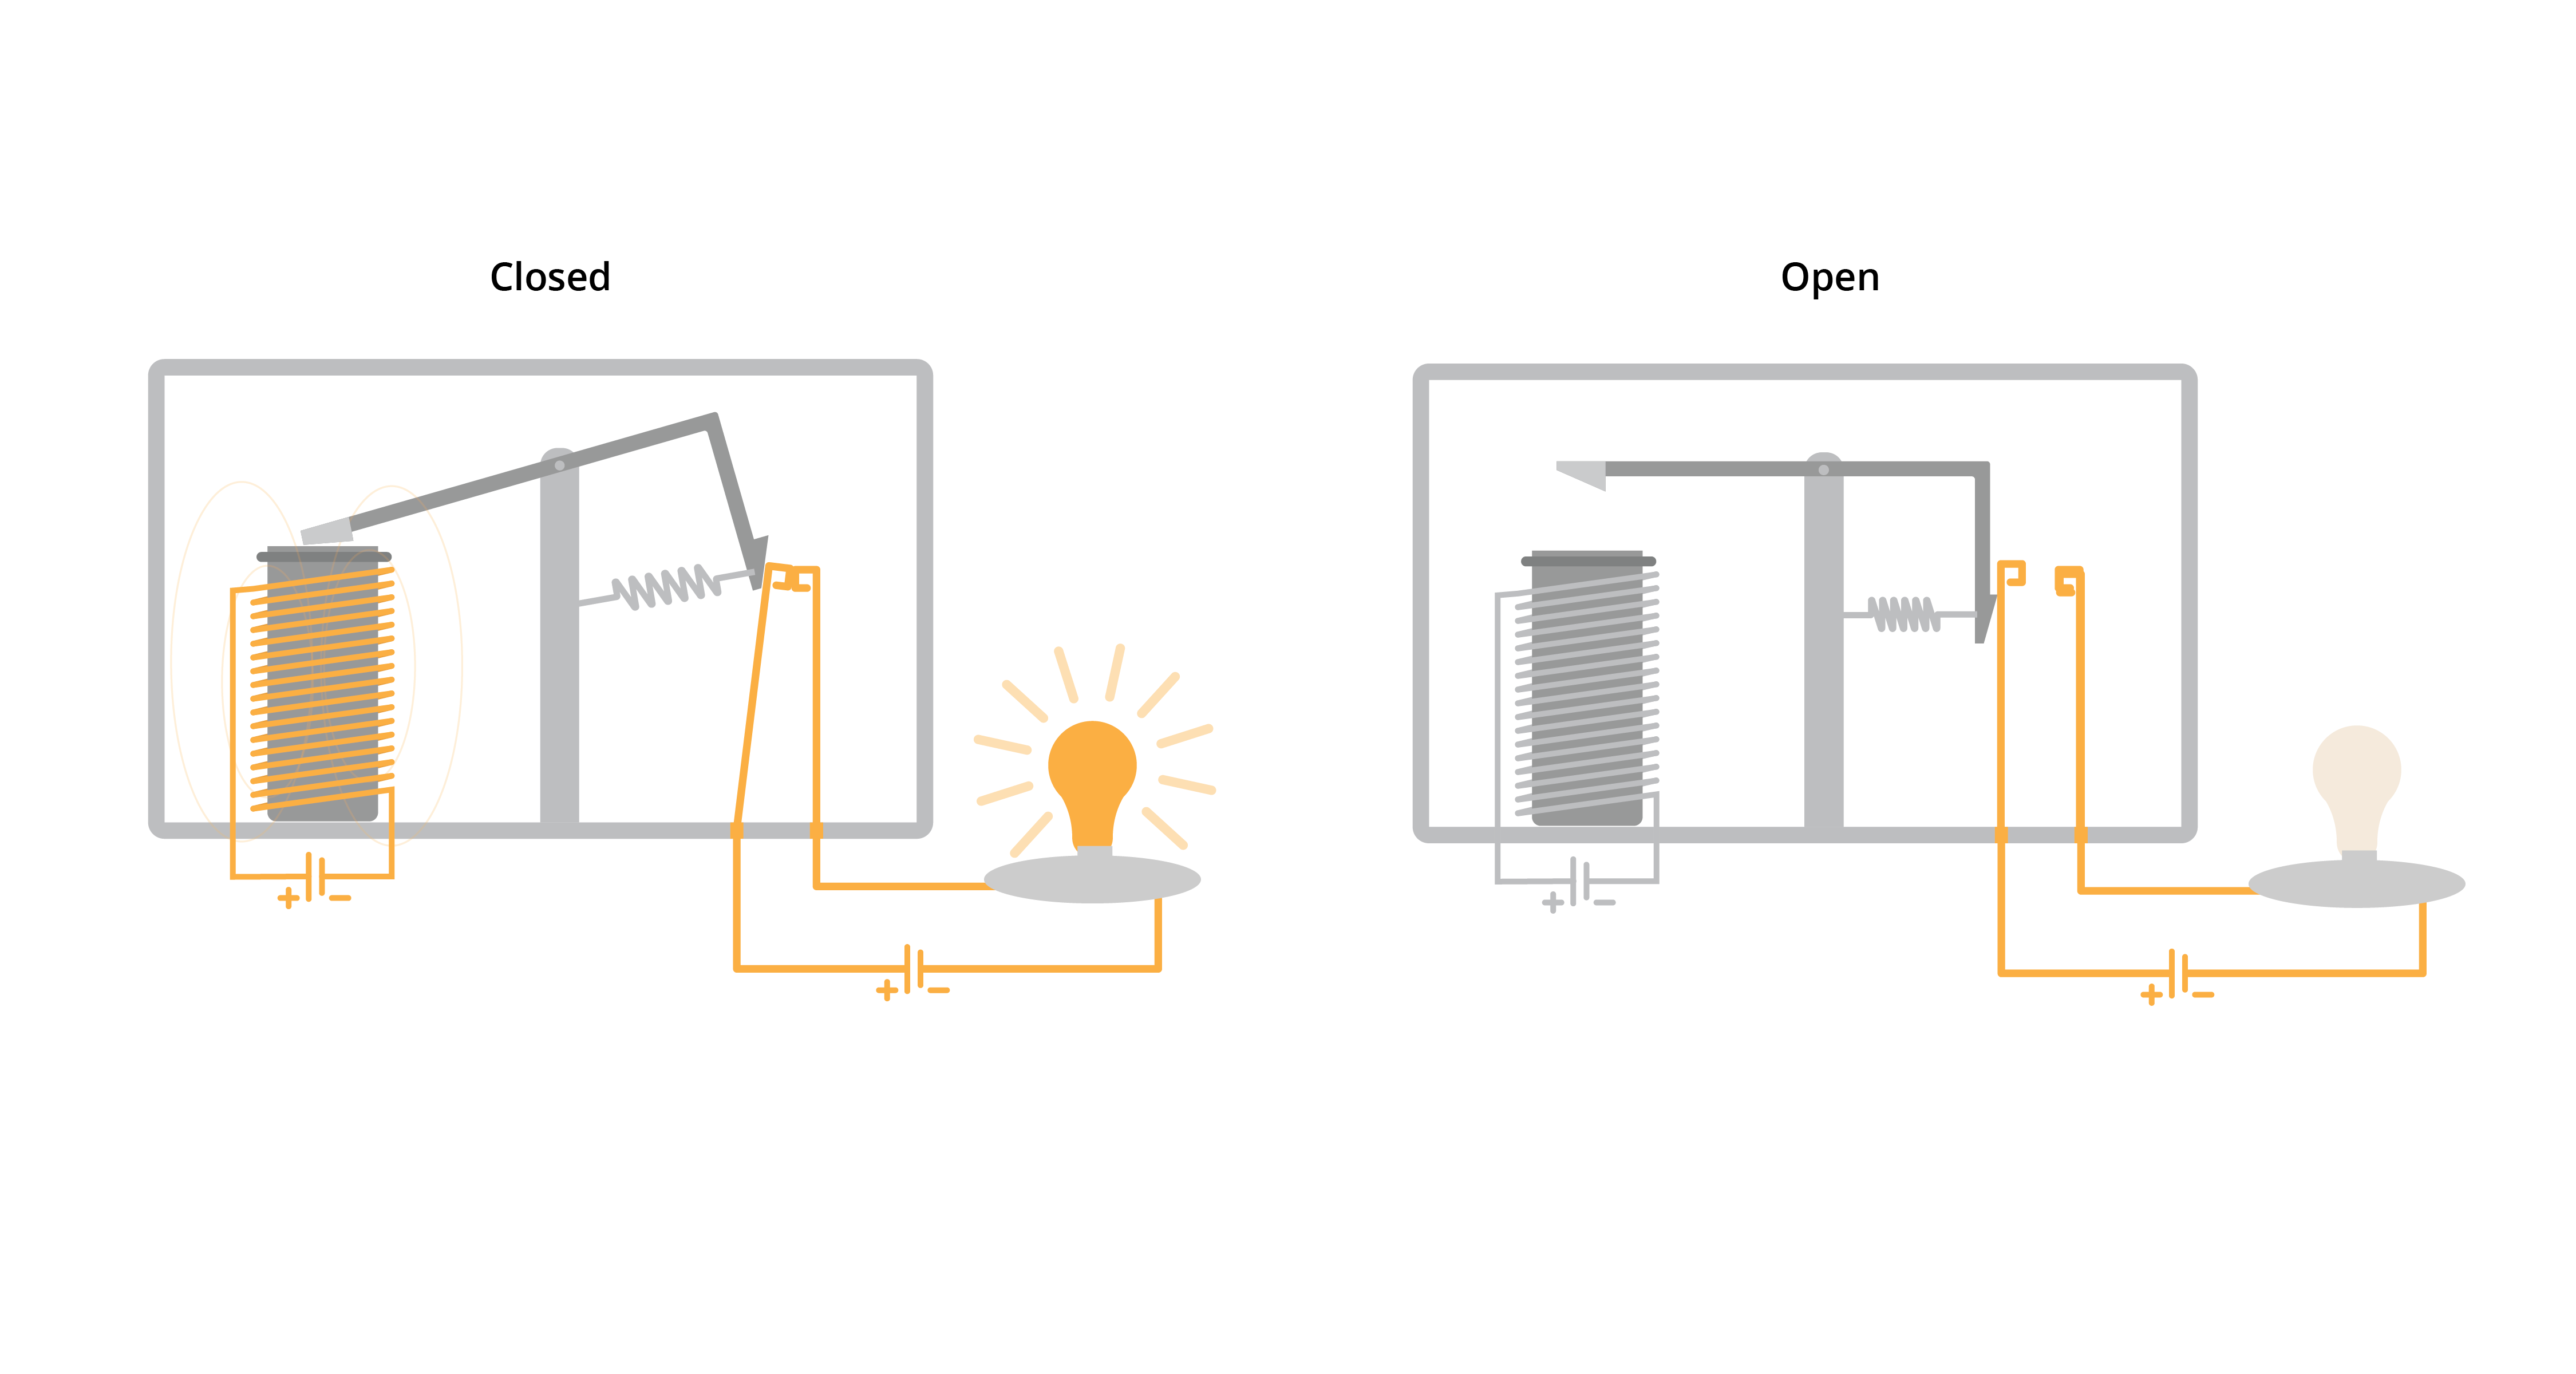
\includegraphics[width=.75\textwidth]{relayFull.png}

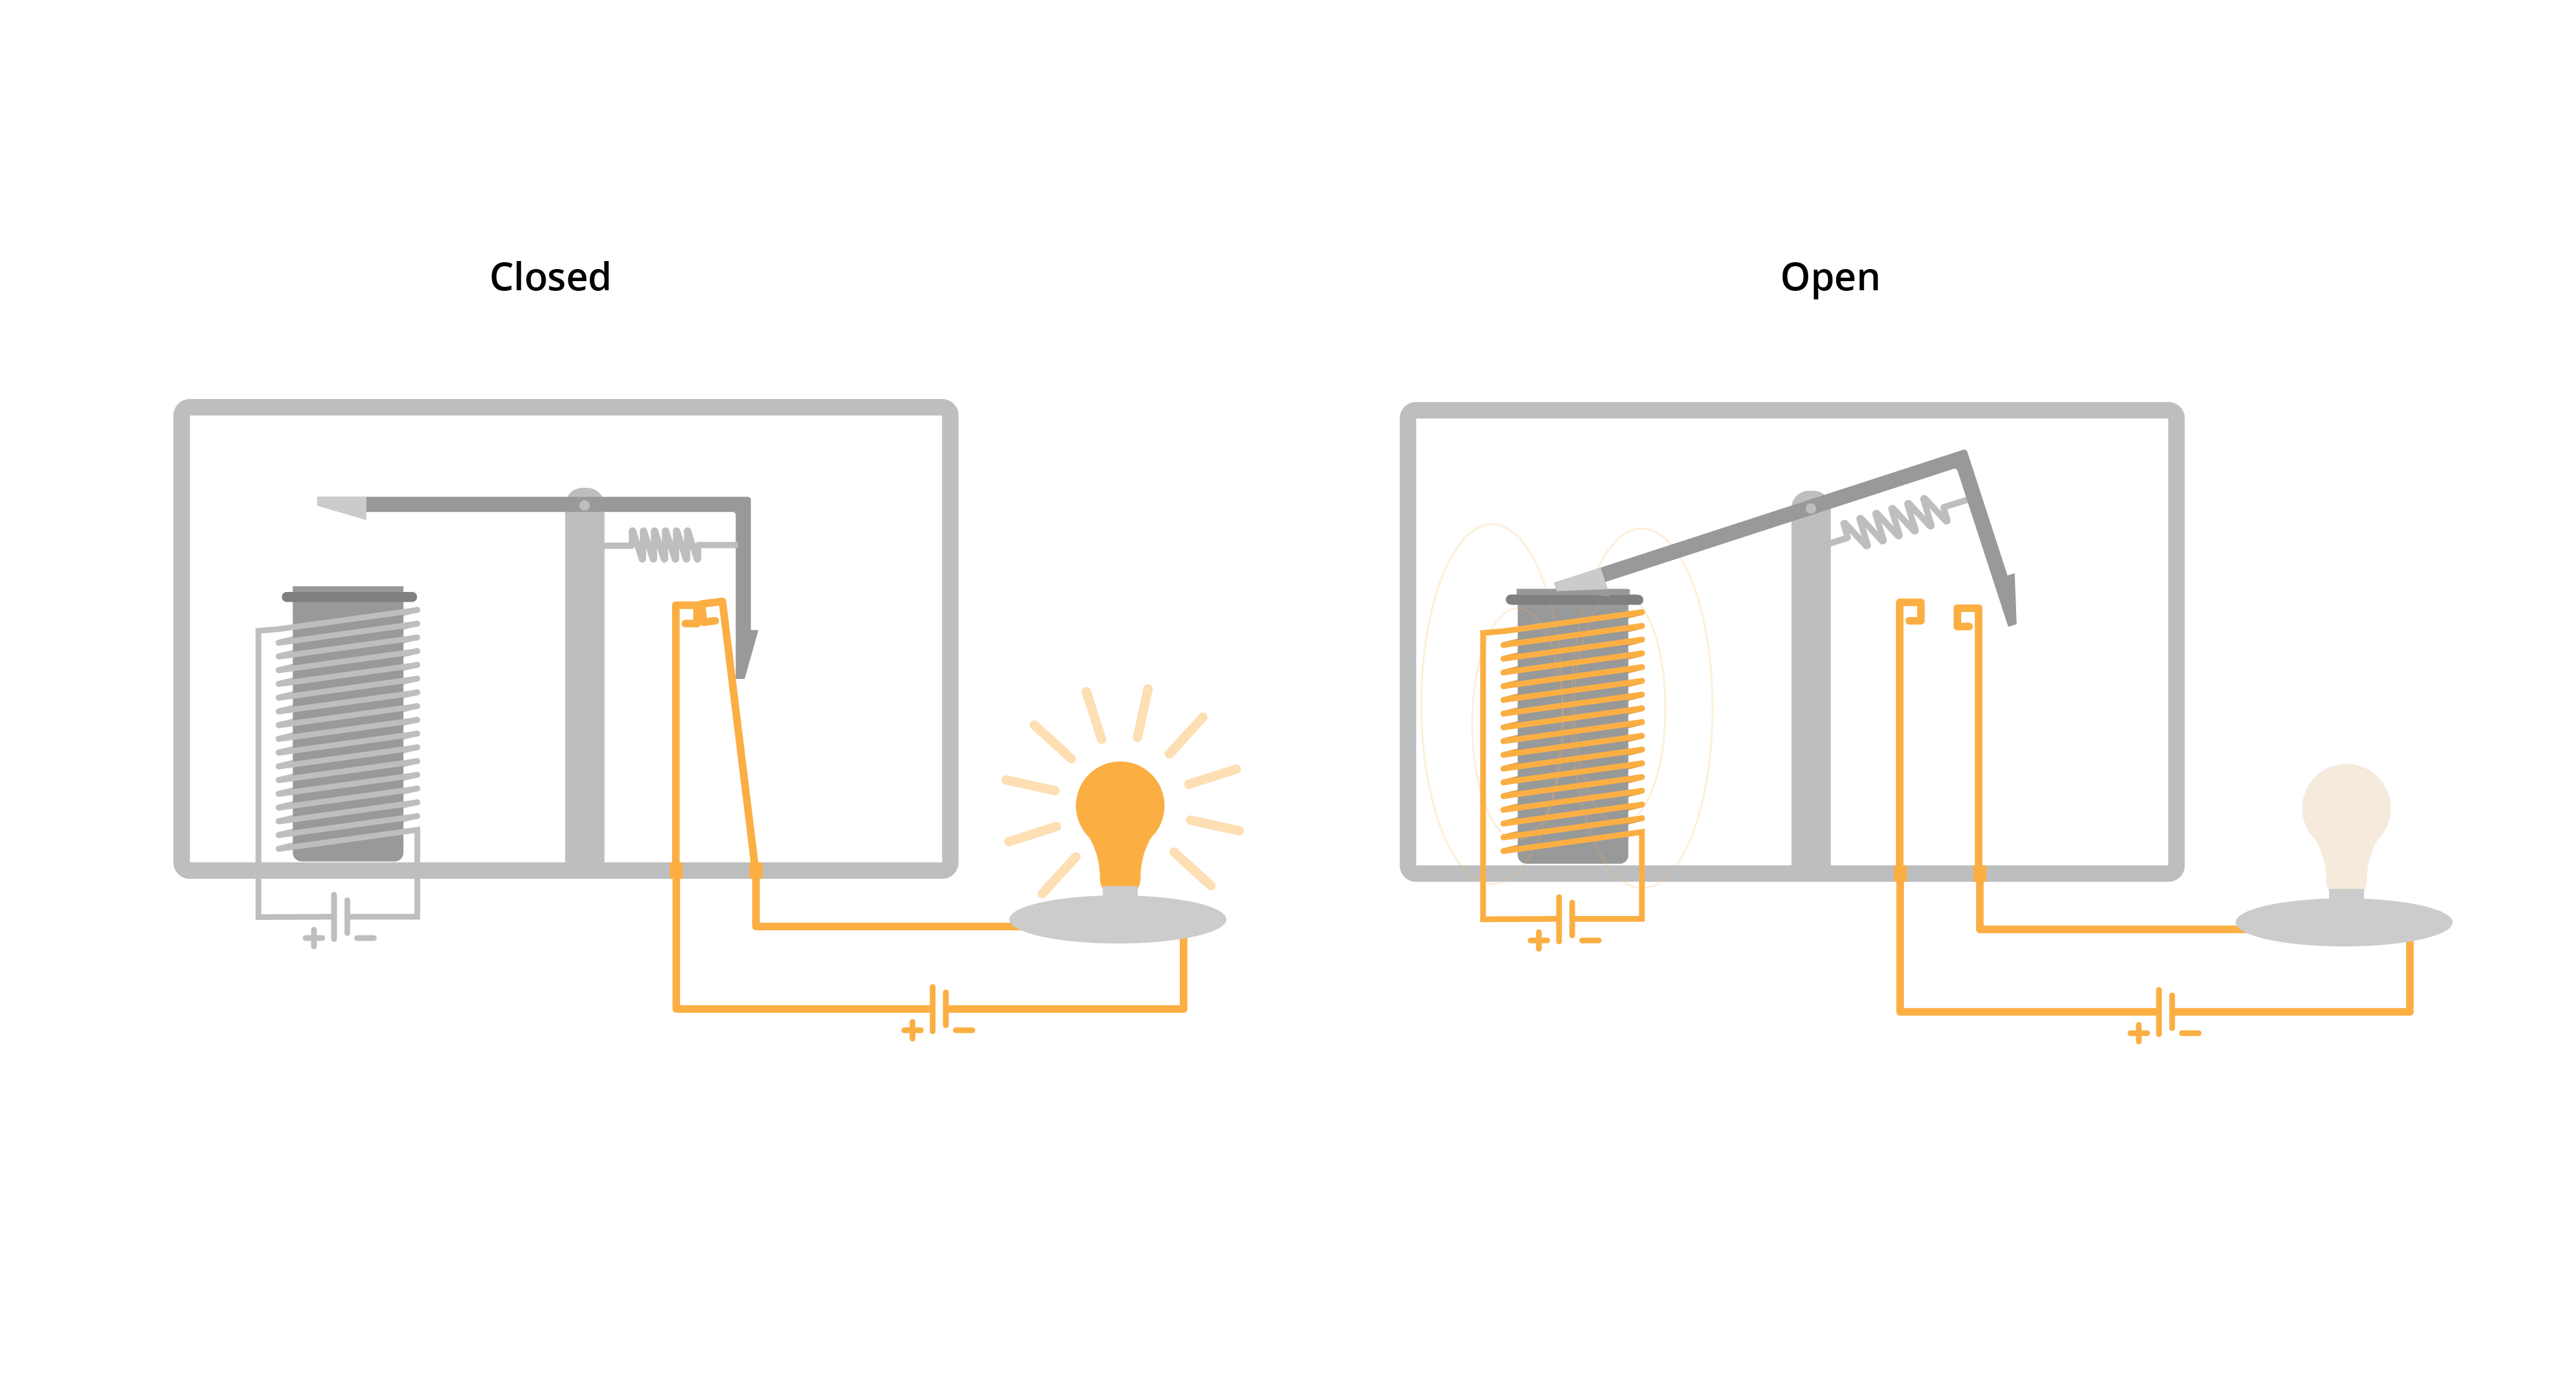
\includegraphics[width=.75\textwidth]{relayFull2.png}

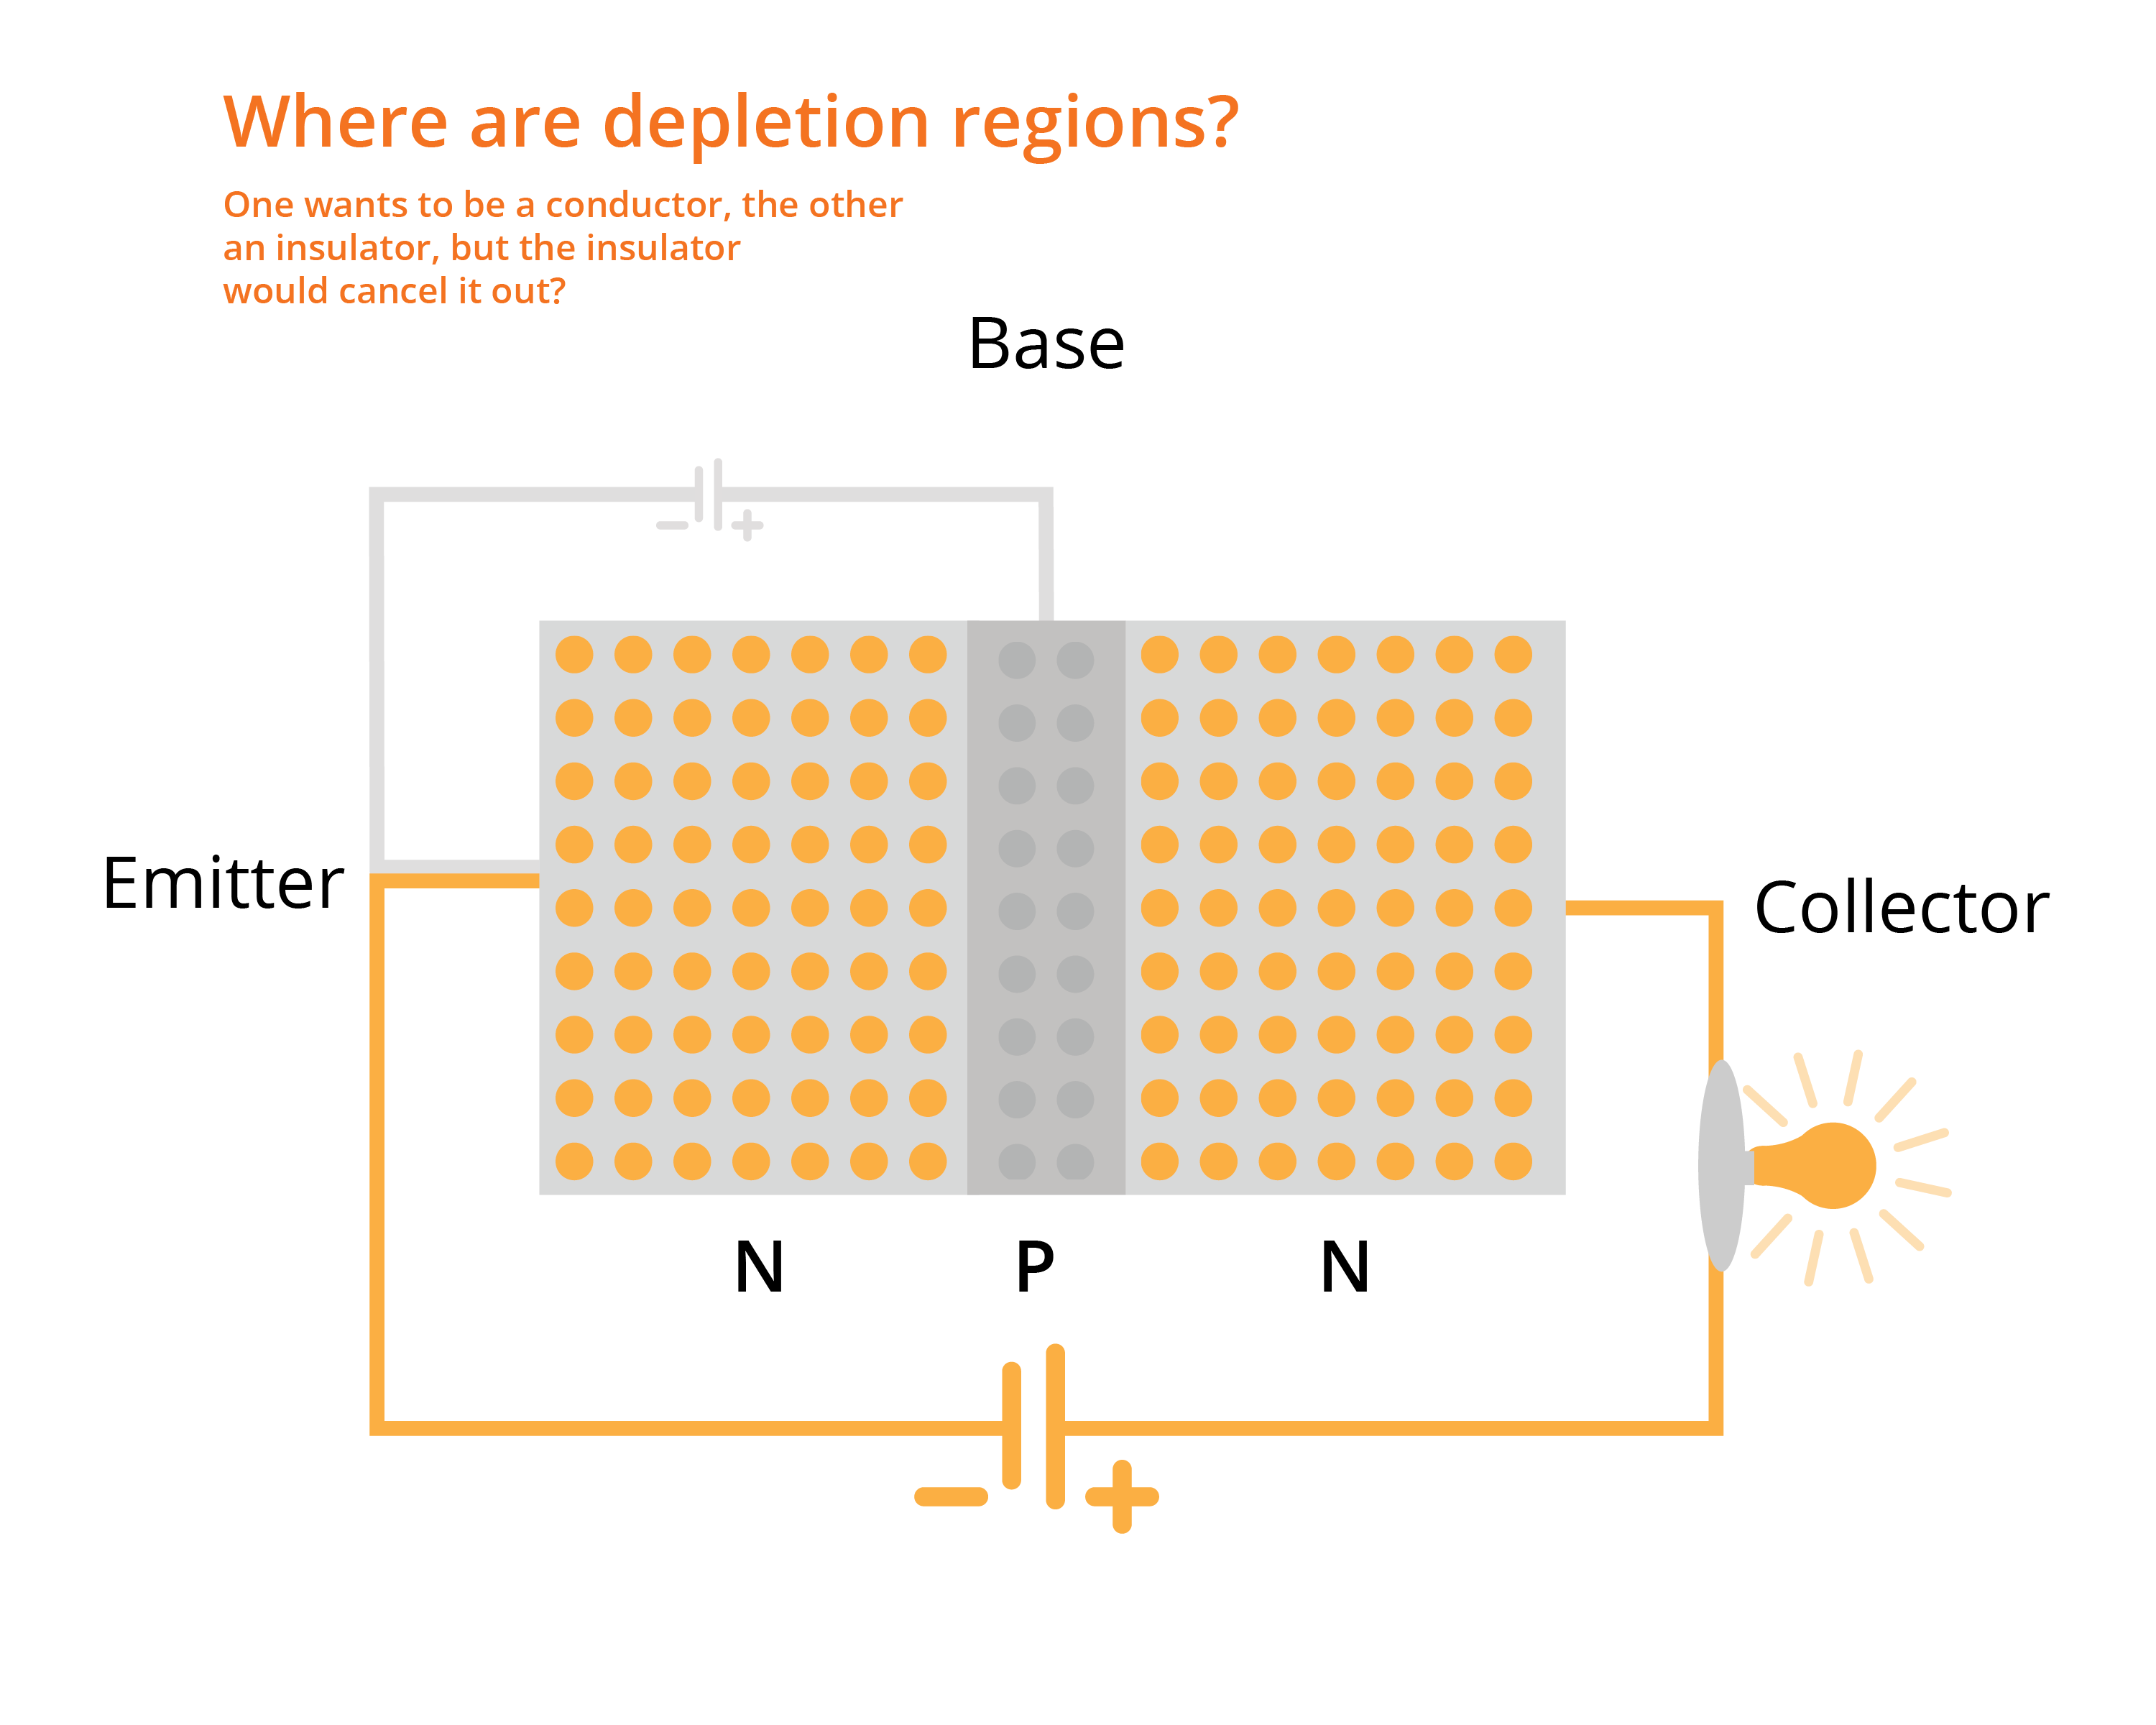
\includegraphics[width=.75\textwidth]{transistorAtom-45.png}

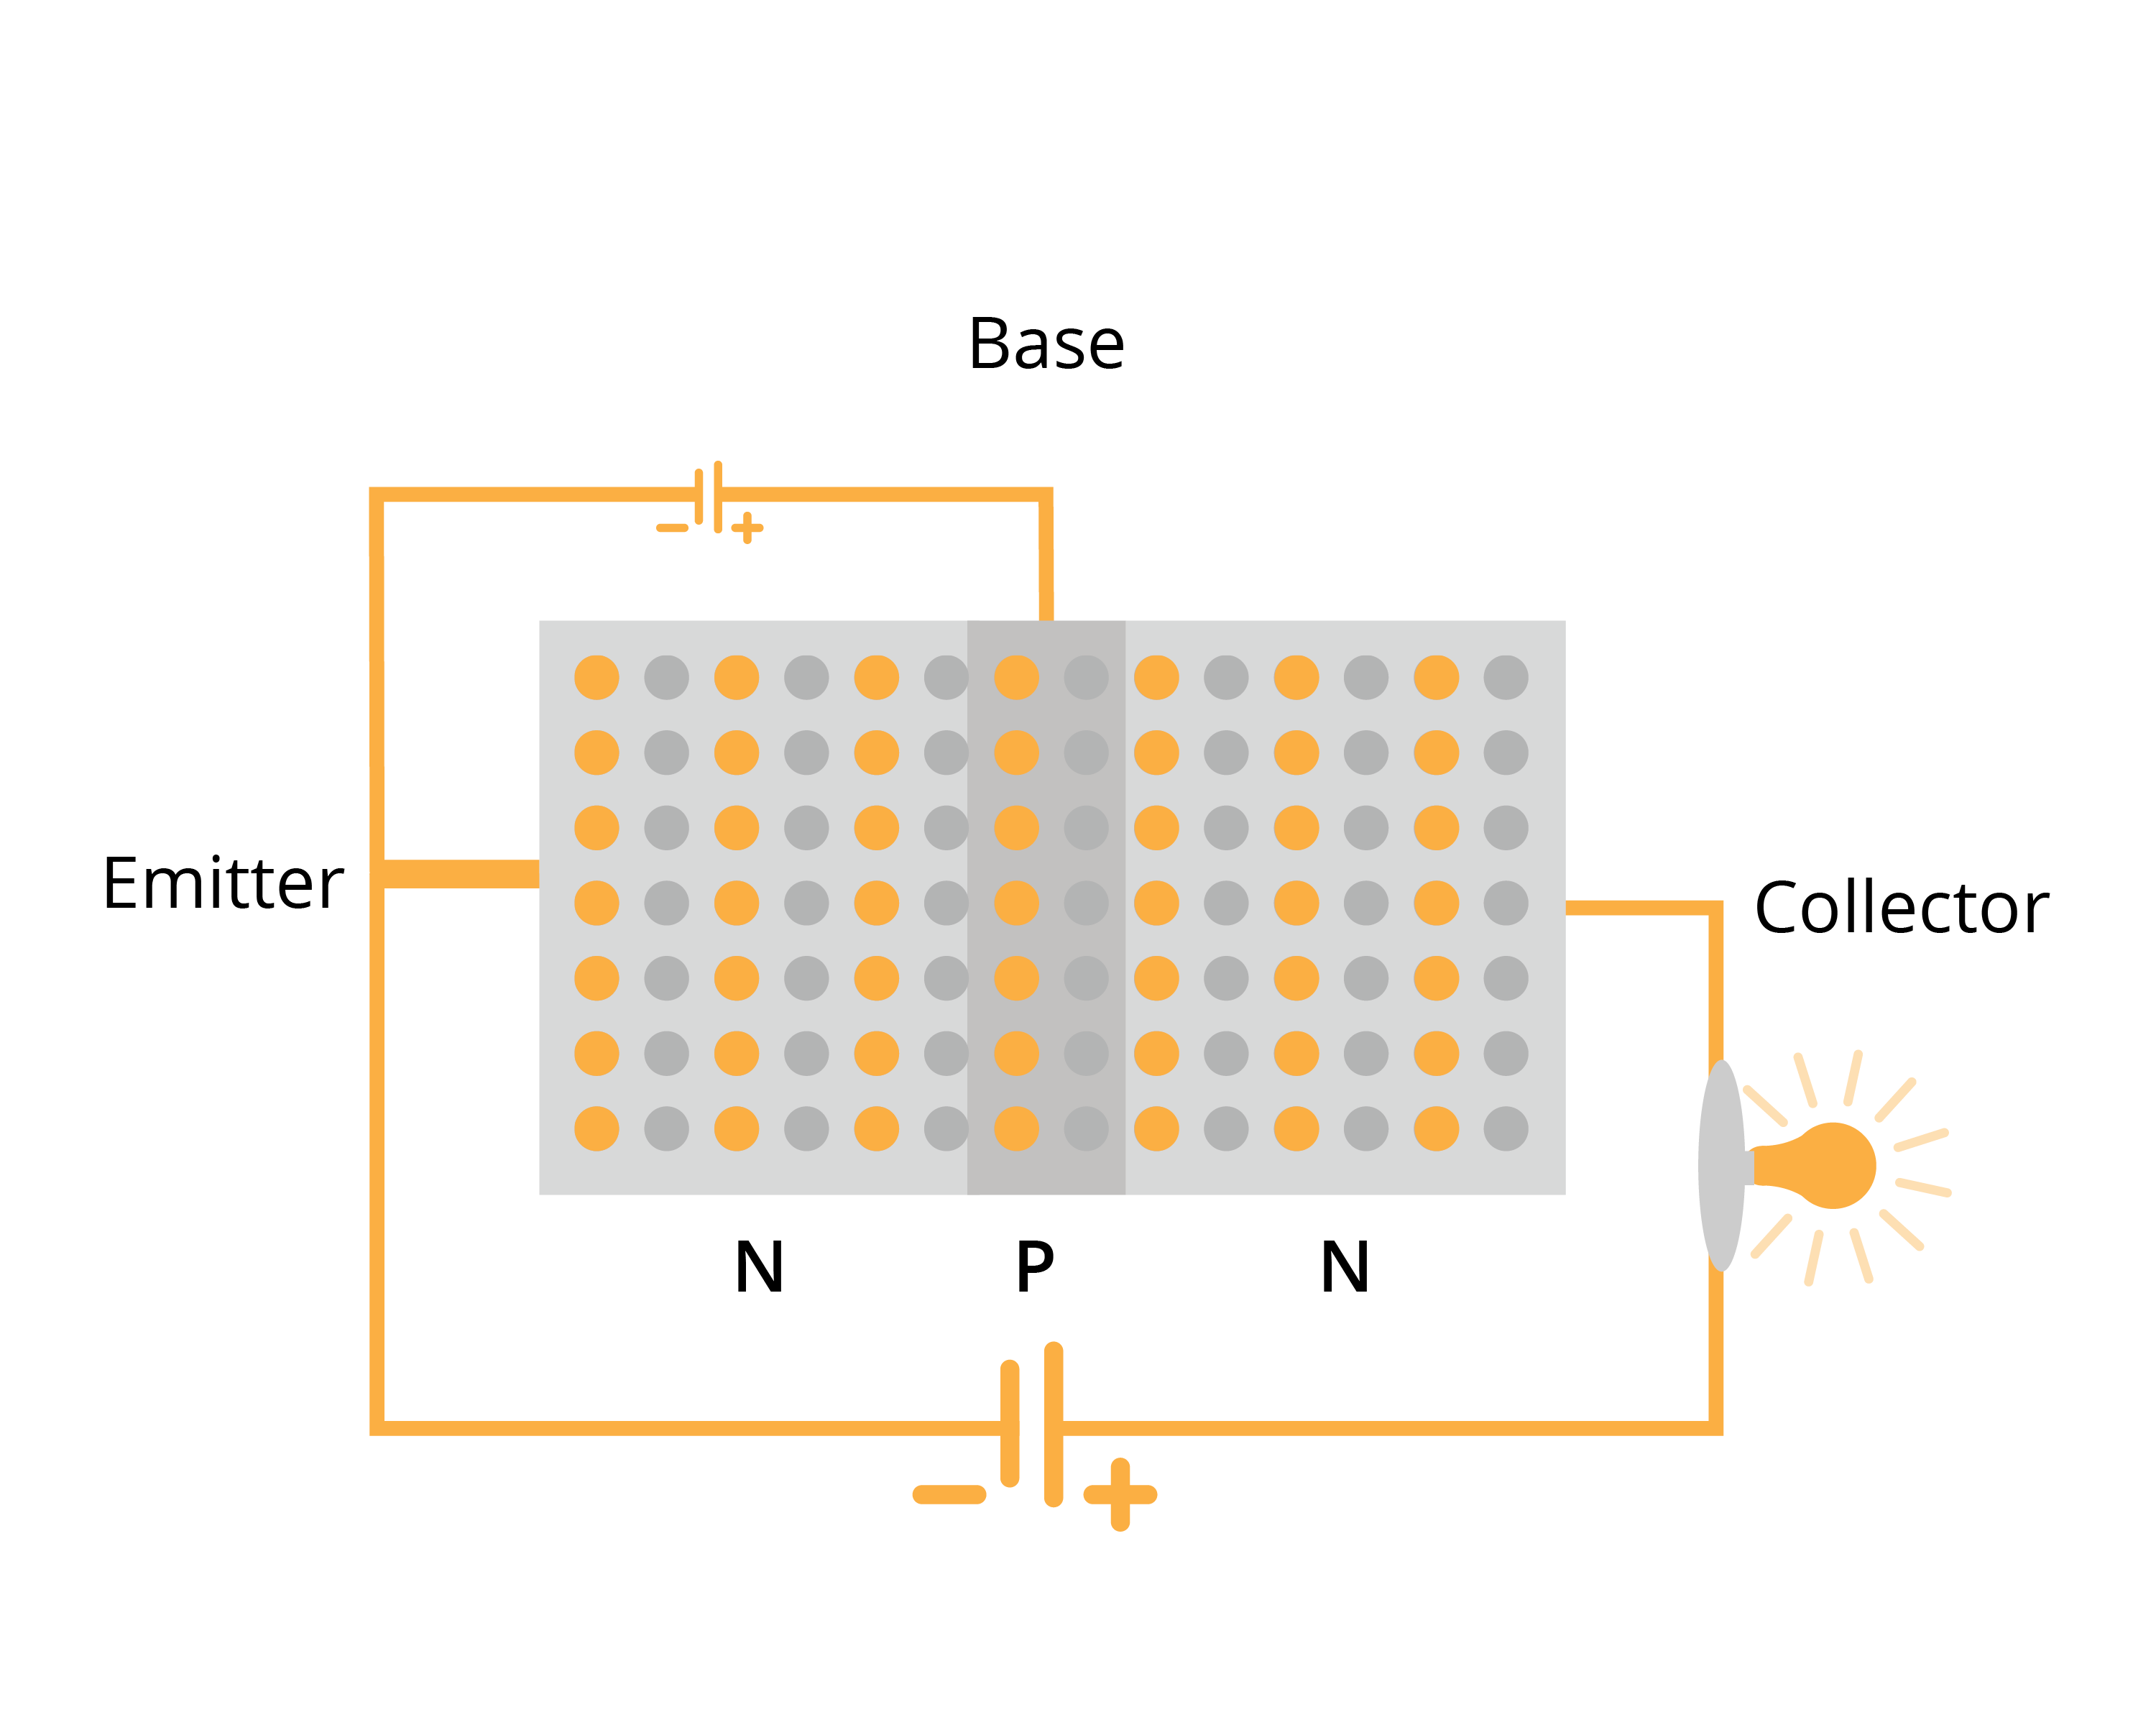
\includegraphics[width=.75\textwidth]{transistorAtom-46.png}

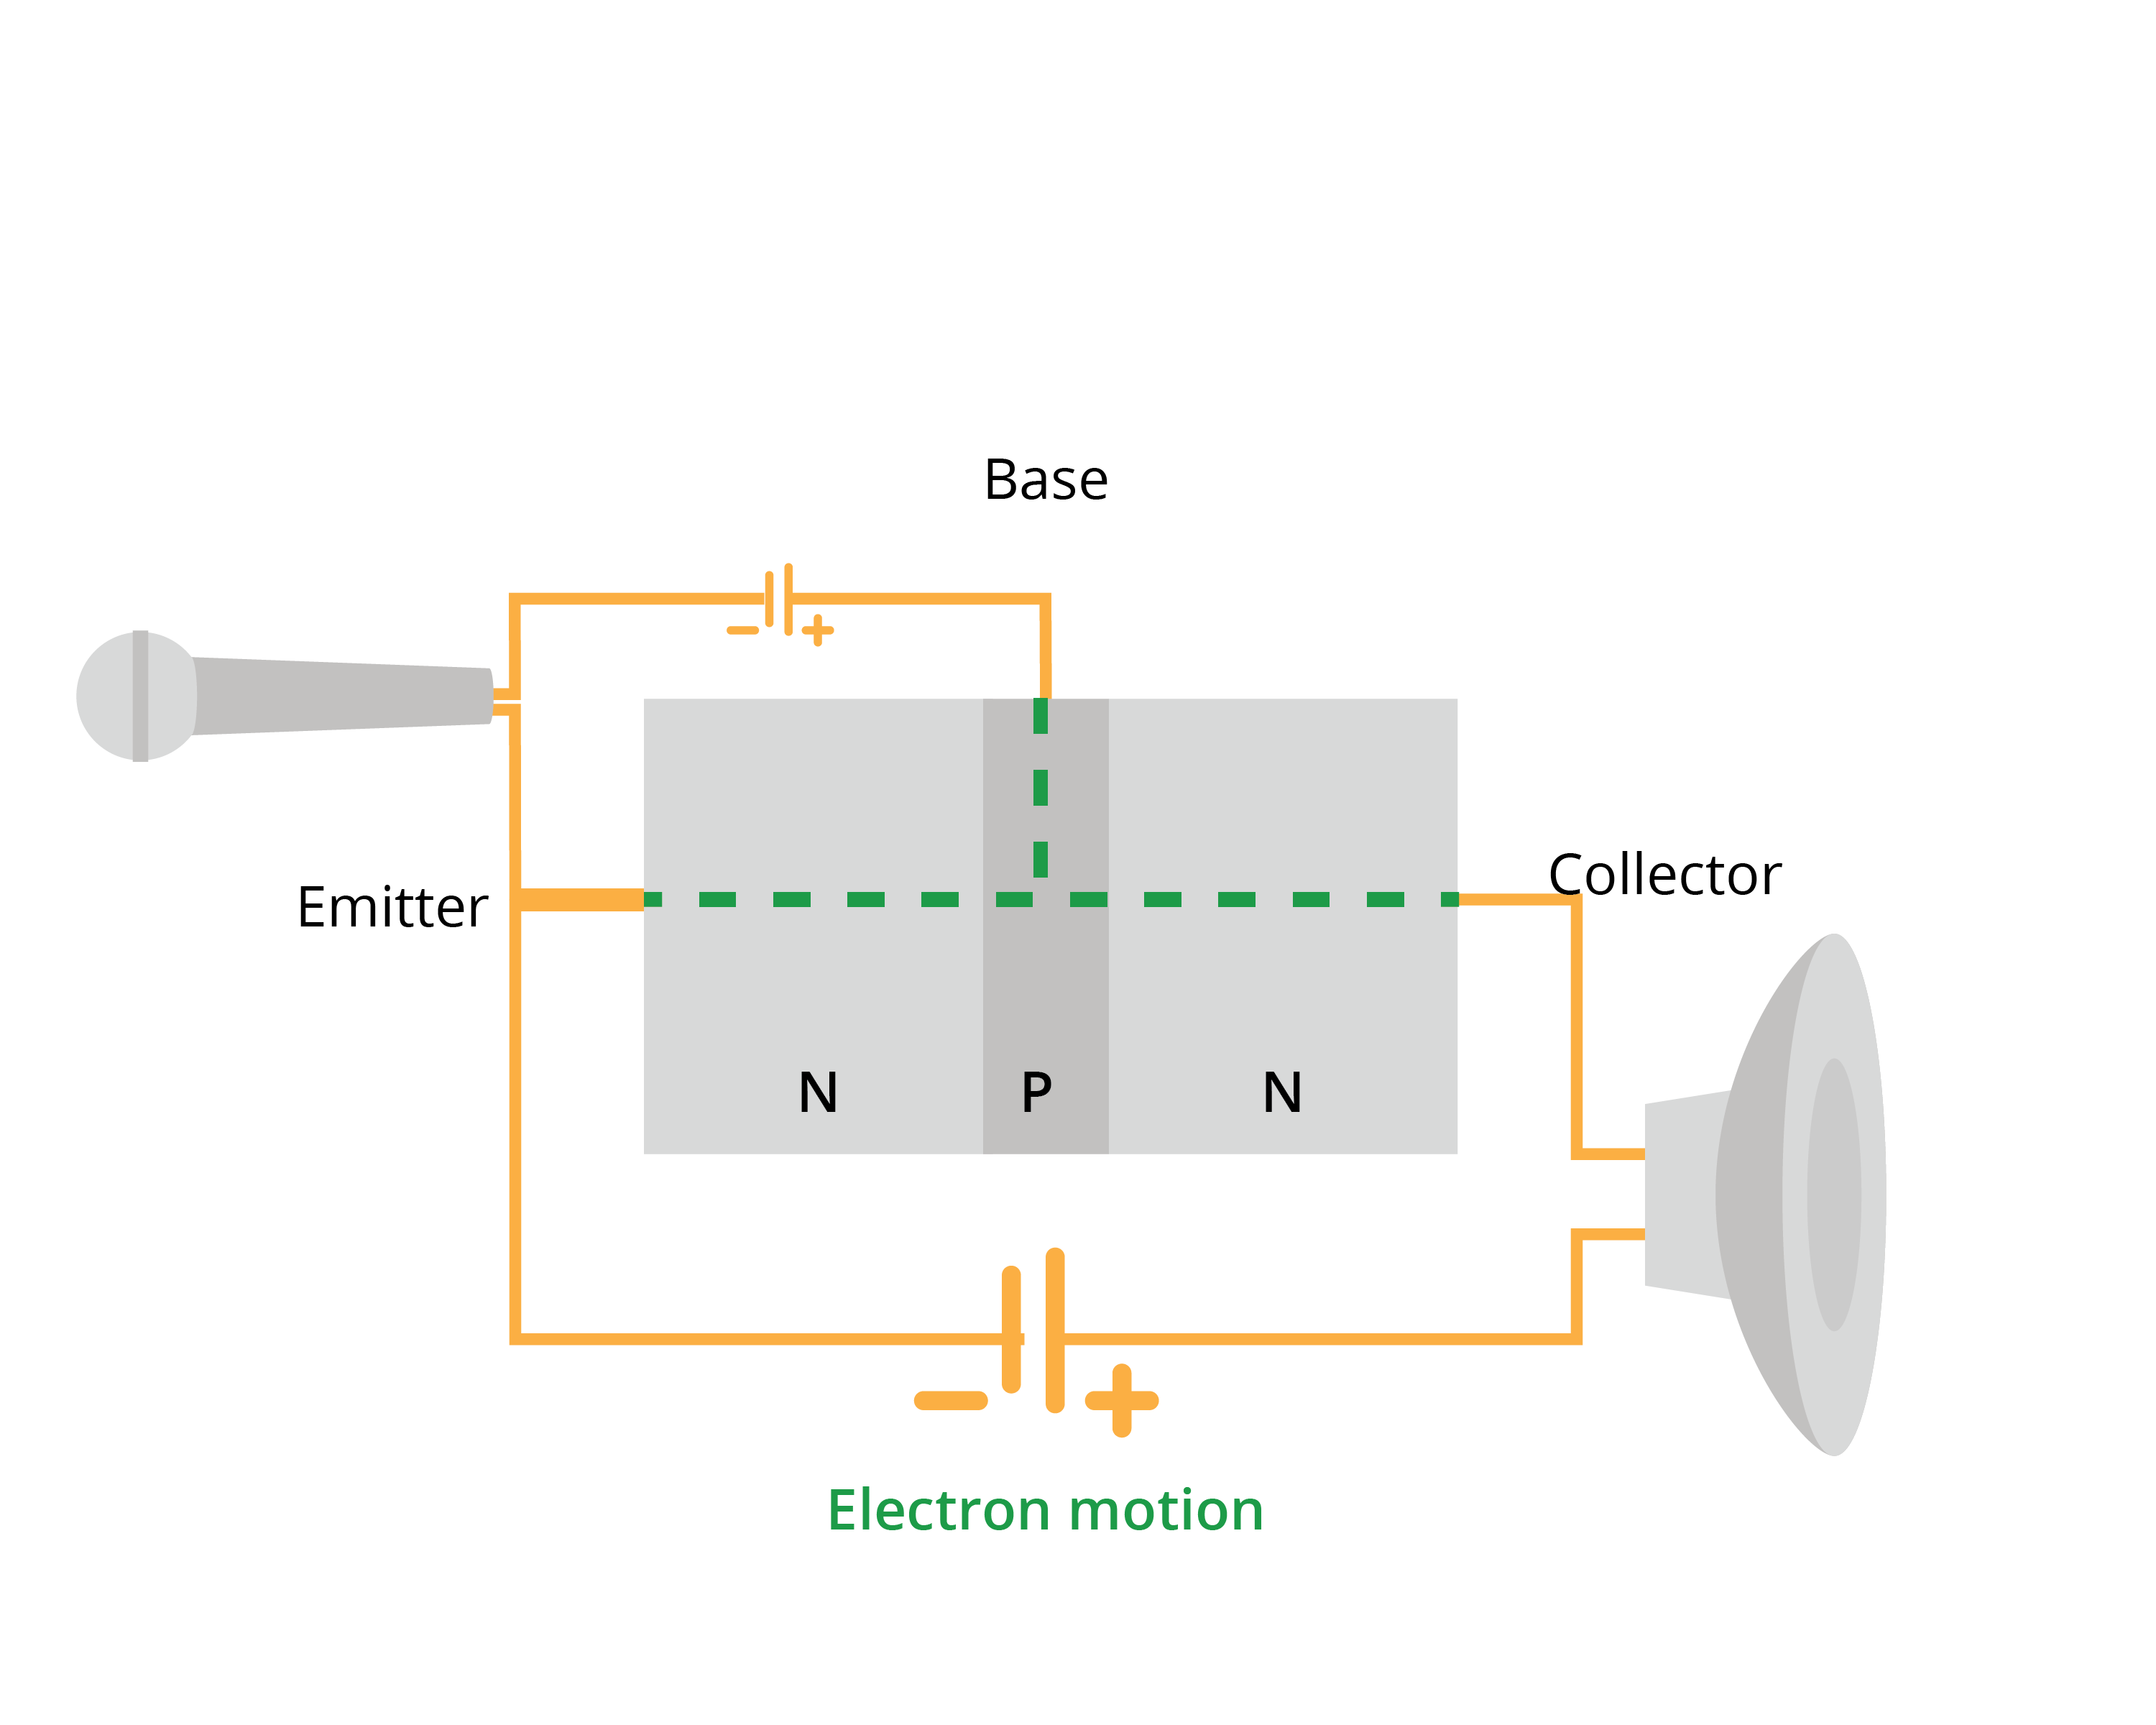
\includegraphics[width=.75\textwidth]{transistorAmp.png}




\begin{circuitikz} \draw
    (0,0) to[battery] (4,0)
    (4,0) -- (4,4)
    (4,4) to[lamp] (0,4)
    (0,4) to[resistor] (0,0);
  
\end{circuitikz}
\end{document}